%%%%%%%%%%%%%%%%%%%%%%%%%%%%%%%%%%%%%%%%%
% Masters/Doctoral Thesis 
% LaTeX Template
% Version 2.4 (22/11/16)
%
% This template has been downloaded from:
% http://www.LaTeXTemplates.com
%
% Version 2.x major modifications by:
% Vel (vel@latextemplates.com)
%
% This template is based on a template by:
% Steve Gunn (http://users.ecs.soton.ac.uk/srg/softwaretools/document/templates/)
% Sunil Patel (http://www.sunilpatel.co.uk/thesis-template/)
%
% Template license:
% CC BY-NC-SA 3.0 (http://creativecommons.org/licenses/by-nc-sa/3.0/)
%
%%%%%%%%%%%%%%%%%%%%%%%%%%%%%%%%%%%%%%%%%

%----------------------------------------------------------------------------------------
%	PACKAGES AND OTHER DOCUMENT CONFIGURATIONS
%----------------------------------------------------------------------------------------

\documentclass[
11pt, % The default document font size, options: 10pt, 11pt, 12pt
oneside, % Two side (alternating margins) for binding by default, uncomment to switch to one side
spanish, % ngerman for German
singlespacing, % Single line spacing, alternatives: onehalfspacing or doublespacing
%draft, % Uncomment to enable draft mode (no pictures, no links, overfull hboxes indicated)
%nolistspacing, % If the document is onehalfspacing or doublespacing, uncomment this to set spacing in lists to single
%liststotoc, % Uncomment to add the list of figures/tables/etc to the table of contents
%toctotoc, % Uncomment to add the main table of contents to the table of contents
parskip, % Uncomment to add space between paragraphs
%nohyperref, % Uncomment to not load the hyperref package
headsepline, % Uncomment to get a line under the header
%chapterinoneline, % Uncomment to place the chapter title next to the number on one line
%consistentlayout, % Uncomment to change the layout of the declaration, abstract and acknowledgements pages to match the default layout
]{MastersDoctoralThesis} % The class file specifying the document structure

\usepackage[utf8]{inputenc} % Required for inputting international characters
\usepackage[T1]{fontenc} % Output font encoding for international characters

\usepackage{palatino} % Use the Palatino font by default

\usepackage[backend=biber,style=authoryear,natbib=true]{biblatex} % Use the bibtex backend with the authoryear citation style (which resembles APA)

\addbibresource{bibliografia.bib} % The filename of the bibliography

\usepackage[autostyle=true]{csquotes} % Required to generate language-dependent quotes in the bibliography

%\setlength{\parskip}{2mm}
%----------------------------------------------------------------------------------------
%	MARGIN SETTINGS
%----------------------------------------------------------------------------------------

\geometry{
	paper=a4paper, % Change to letterpaper for US letter
	inner=2.5cm, % Inner margin
	outer=3.8cm, % Outer margin
	bindingoffset=.5cm, % Binding offset
	top=1.5cm, % Top margin
	bottom=1.5cm, % Bottom margin
	%showframe, % Uncomment to show how the type block is set on the page
}

%----------------------------------------------------------------------------------------
%	THESIS INFORMATION
%----------------------------------------------------------------------------------------

\thesistitle{Thesis Title} % Your thesis title, this is used in the title and abstract, print it elsewhere with \ttitle
\supervisor{Dr. James \textsc{Smith}} % Your supervisor's name, this is used in the title page, print it elsewhere with \supname
\examiner{} % Your examiner's name, this is not currently used anywhere in the template, print it elsewhere with \examname
\degree{Doctor of Philosophy} % Your degree name, this is used in the title page and abstract, print it elsewhere with \degreename
\author{John \textsc{Smith}} % Your name, this is used in the title page and abstract, print it elsewhere with \authorname
\addresses{} % Your address, this is not currently used anywhere in the template, print it elsewhere with \addressname

\subject{Biological Sciences} % Your subject area, this is not currently used anywhere in the template, print it elsewhere with \subjectname
\keywords{} % Keywords for your thesis, this is not currently used anywhere in the template, print it elsewhere with \keywordnames
\university{\href{http://www.university.com}{University Name}} % Your university's name and URL, this is used in the title page and abstract, print it elsewhere with \univname
\department{\href{http://department.university.com}{Department or School Name}} % Your department's name and URL, this is used in the title page and abstract, print it elsewhere with \deptname
\group{\href{http://researchgroup.university.com}{Research Group Name}} % Your research group's name and URL, this is used in the title page, print it elsewhere with \groupname
\faculty{\href{http://faculty.university.com}{Faculty Name}} % Your faculty's name and URL, this is used in the title page and abstract, print it elsewhere with \facname

\AtBeginDocument{
\hypersetup{pdftitle=\ttitle} % Set the PDF's title to your title
\hypersetup{pdfauthor=\authorname} % Set the PDF's author to your name
\hypersetup{pdfkeywords=\keywordnames} % Set the PDF's keywords to your keywords
}

\begin{document}

\frontmatter % Use roman page numbering style (i, ii, iii, iv...) for the pre-content pages

\pagestyle{plain} % Default to the plain heading style until the thesis style is called for the body content

%----------------------------------------------------------------------------------------
%	TITLE PAGE
%----------------------------------------------------------------------------------------



%----------------------------------------------------------------------------------------
%	DECLARATION PAGE
%----------------------------------------------------------------------------------------



%----------------------------------------------------------------------------------------
%	QUOTATION PAGE
%----------------------------------------------------------------------------------------



%----------------------------------------------------------------------------------------
%	ABSTRACT PAGE
%----------------------------------------------------------------------------------------



%----------------------------------------------------------------------------------------
%	ACKNOWLEDGEMENTS
%----------------------------------------------------------------------------------------



%----------------------------------------------------------------------------------------
%	LIST OF CONTENTS/FIGURES/TABLES PAGES
%----------------------------------------------------------------------------------------

%\tableofcontents % Prints the main table of contents
%\listoffigures % Prints the list of figures
%\listoftables % Prints the list of tables

%----------------------------------------------------------------------------------------
%	ABBREVIATIONS
%----------------------------------------------------------------------------------------



%----------------------------------------------------------------------------------------
%	PHYSICAL CONSTANTS/OTHER DEFINITIONS
%----------------------------------------------------------------------------------------


%----------------------------------------------------------------------------------------
%	SYMBOLS
%----------------------------------------------------------------------------------------

%----------------------------------------------------------------------------------------
%	DEDICATION
%----------------------------------------------------------------------------------------


%----------------------------------------------------------------------------------------
%	THESIS CONTENT - CHAPTERS
%----------------------------------------------------------------------------------------

\mainmatter % Begin numeric (1,2,3...) page numbering

\pagestyle{thesis} % Return the page headers back to the "thesis" style

% Include the chapters of the thesis as separate files from the Chapters folder
% Uncomment the lines as you write the chapters

% Chapter Template

\chapter{Introducción} % Main chapter title

\label{Chapter1} % Change X to a consecutive number; for referencing this chapter elsewhere, use \ref{ChapterX}

En este primer capítulo se propone dar una visión general del contexto en que se encuadra el proyecto fin de carrera, que es: la visión artificial. Dentro de ésta se abordará el problema al que vamos a hacer frente: La autolocalización visual, o dicho de otro modo, la estimación de la posición y orientación de un sensor con seis grados de libertad (SLAM).

%-----------------------------------
%	SECTION Visión artificial
%-----------------------------------
\section{Visión artificial}

El ser humano no es consciente del proceso neuronal que tiene lugar en nuestro cerebro con el simple hecho de andar o coger un objeto. Se podría decir que tenemos un super ordenador conectado a los órganos sensoriales capaces de recoger muchísima información y procesarla en un tiempo récord.

Desde la antiguedad ya se estuvo pensando en reproducir las habilidades humanas en algún tipo de máquina, la noción de concebir la mente humana como algún tipo de mecanismo no es reciente es referida en célebres filósofos, sin embargo, no es hasta 1950 y con la noción de la computación cuando se introduce la IA (Inteligencia Artificial) por el científico Alan Turing en su artículo \textit{Maquinaria Computacional e Inteligencia} y donde se empieza a coger interés por este campo que será el precursor de una gran cantidad de desarrollos e innovaciones.

Dentro del campo de la inteligencia artificial se puede definir \textbf{visión artificial} como la disciplina científica que incluye métodos para adquirir, procesar y analizar imágenes con el fin de producir información que pueda ser tratada por una máquina ofreciendo soluciones a problemas del mundo real.

Una manera simple de comprender este sistema es basarnos en nuestra propia experiencia. Los humanos usamos nuestros sentidos, especialmente la visión, para comprender el mundo que nos rodea, y la visión artificial busca producir ese mismo efecto en máquinas.

Cada vez son más los dispositivos electrónicos que llevan incorporada al menos una cámara; \textit{smartphones}, ordenadores portátiles, \textit{tablets}, consolas de videojuegos... Debido a la gran cantidad de información que se puede extraer de las imágenes, el bajo coste, el reducido tamaño de las cámaras y el aumento de capacidad de cómputo de los dispositivos, es un área que ha suscitado el interés por los investigadores, ha crecido enormemente en los últimos años y está cogiendo cada vez más fuerza.

% Dispositivos electrónicos
Podemos ver cada vez más como los dispositivos electrónicos disponen de alguna nueva funcionalidad relacionada con el procesamiento de imágenes (Figura~\ref{fig:Face}), como puede ser el reconocimiento facial que incorporan algunos smartphones o tablets para desbloquear el dispositivo o procesado automático de fotos realizadas por la cámara como la que incluye el terminal chino \textbf{Meitu T8} que incorpora un software llamado \textit{AI Beautification} para embellecer las imágenes. \footnote{https://www.cnet.com/products/meitu-t8/preview/}

\begin{figure}[th]
\centering
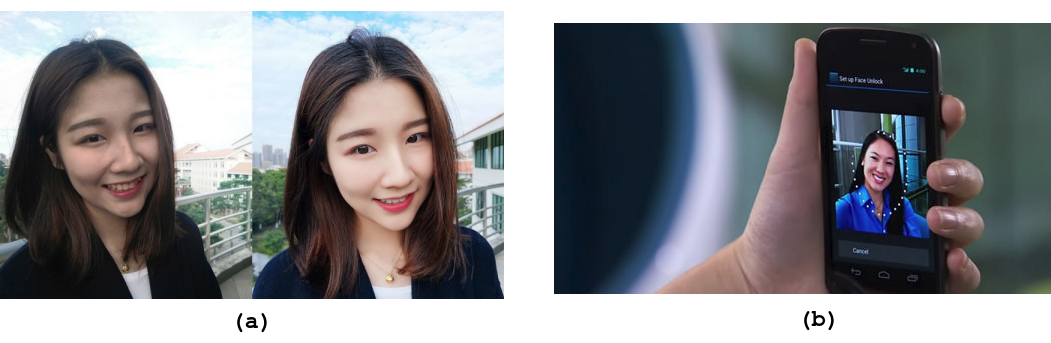
\includegraphics[scale=0.43]{Figures/face.png}
\decoRule
\caption[Embellecimiento de fotos (Meitu T8)]{Embellecimiento de fotos (Meitu T8) (a). Reconocimiento facial (b).}
\label{fig:Face}
\end{figure}

Sin ir más lejos, la reciente aplicación que ha desatado revuelo en las diferentes redes sociales; FaceApp\footnote{https://www.faceapp.com/}. La aplicación disponible tanto para Android e iOS es capaz de añadir sonrisas a las fotos, cambiar de edad o transformar el género de la persona que ha sido fotografiada.

% Medicina
El procesado de imágenes puede llegar a resultar muy útil en otros ámbitos como el de la medicina. Un ejemplo es la radiografía de la Figura~\ref{fig:Medicine} que partiendo de una imágen de muy baja calidad se  pretende  extraer  información  sobre  las  manchas
blancas que aparecen en la misma.

\begin{figure}[th]
\centering
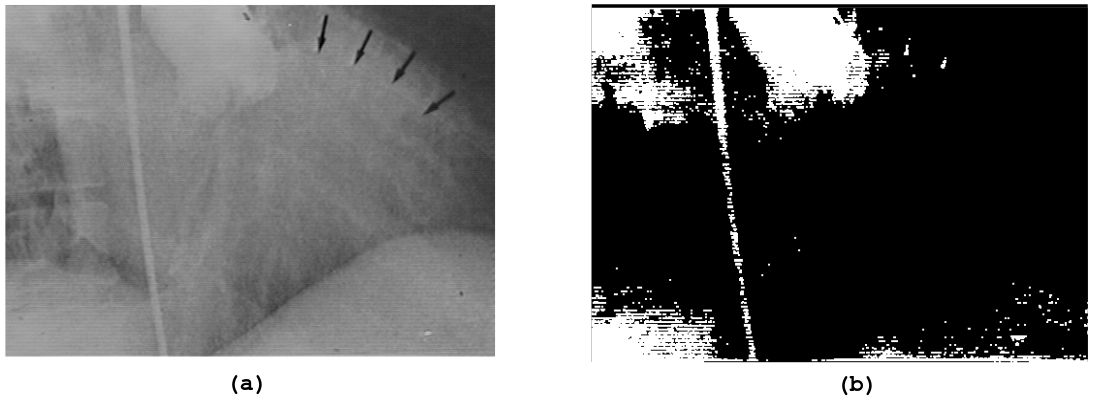
\includegraphics[scale=0.4]{Figures/medicine.png}
\decoRule
\caption[Aplicaciones de radiografía en medicina]{Radiografía inicial, con los puntos a analizar (a), imagen final procesada (b).}
\label{fig:Medicine}
\end{figure}

% Industria
Son numerosas las aplicaciones de visión industrial relacionadas con el entorno de la alimentación. Permiten automatizar el control de calidad para tomar la decisión si un determinado producto cumple el estándar de calidad o no. Un ejemplo es el sistema \textbf{EggInspector}\footnote{http://www.moba.net/page/es/Grading/Moba-Grader-Options/Detection-Systems/Egg-inspector} por la empresa Moba que se utiliza para clasificar huevos de gallina de forma automática. El sistema está compuesto por 6 cámaras suspendidas por encima de la cinta transportadora que con unos complejos algoritmos no solo pueden comprobar si los huevos están rotos o sucios, sino que son capaces de determinar el tipo de rotura y suciedad, una vez determinada la calidad, los que no corresponden a los estándares mínimos, son separados de la línea por un robot.

Siguiendo en la línea de la industria la inspección de embalajes se ha incrementado enormemente con la automatización del proceso y la visión artificial facilitando tareas como la detección del correcto nivel de llenado, verificación de tapones, control de calidad de sellado, lectura de óptica de caracteres (OCR), códigos de barras, verificación de posición, calidad de impresión de las equiquetas, conteo de productos en cajas o \textit{palets}. Algunas de las aplicaciones típicas de la industria del \textit{packaging} están representadas en la Figura~\ref{fig:Industry}.

\begin{figure}[th]
\centering
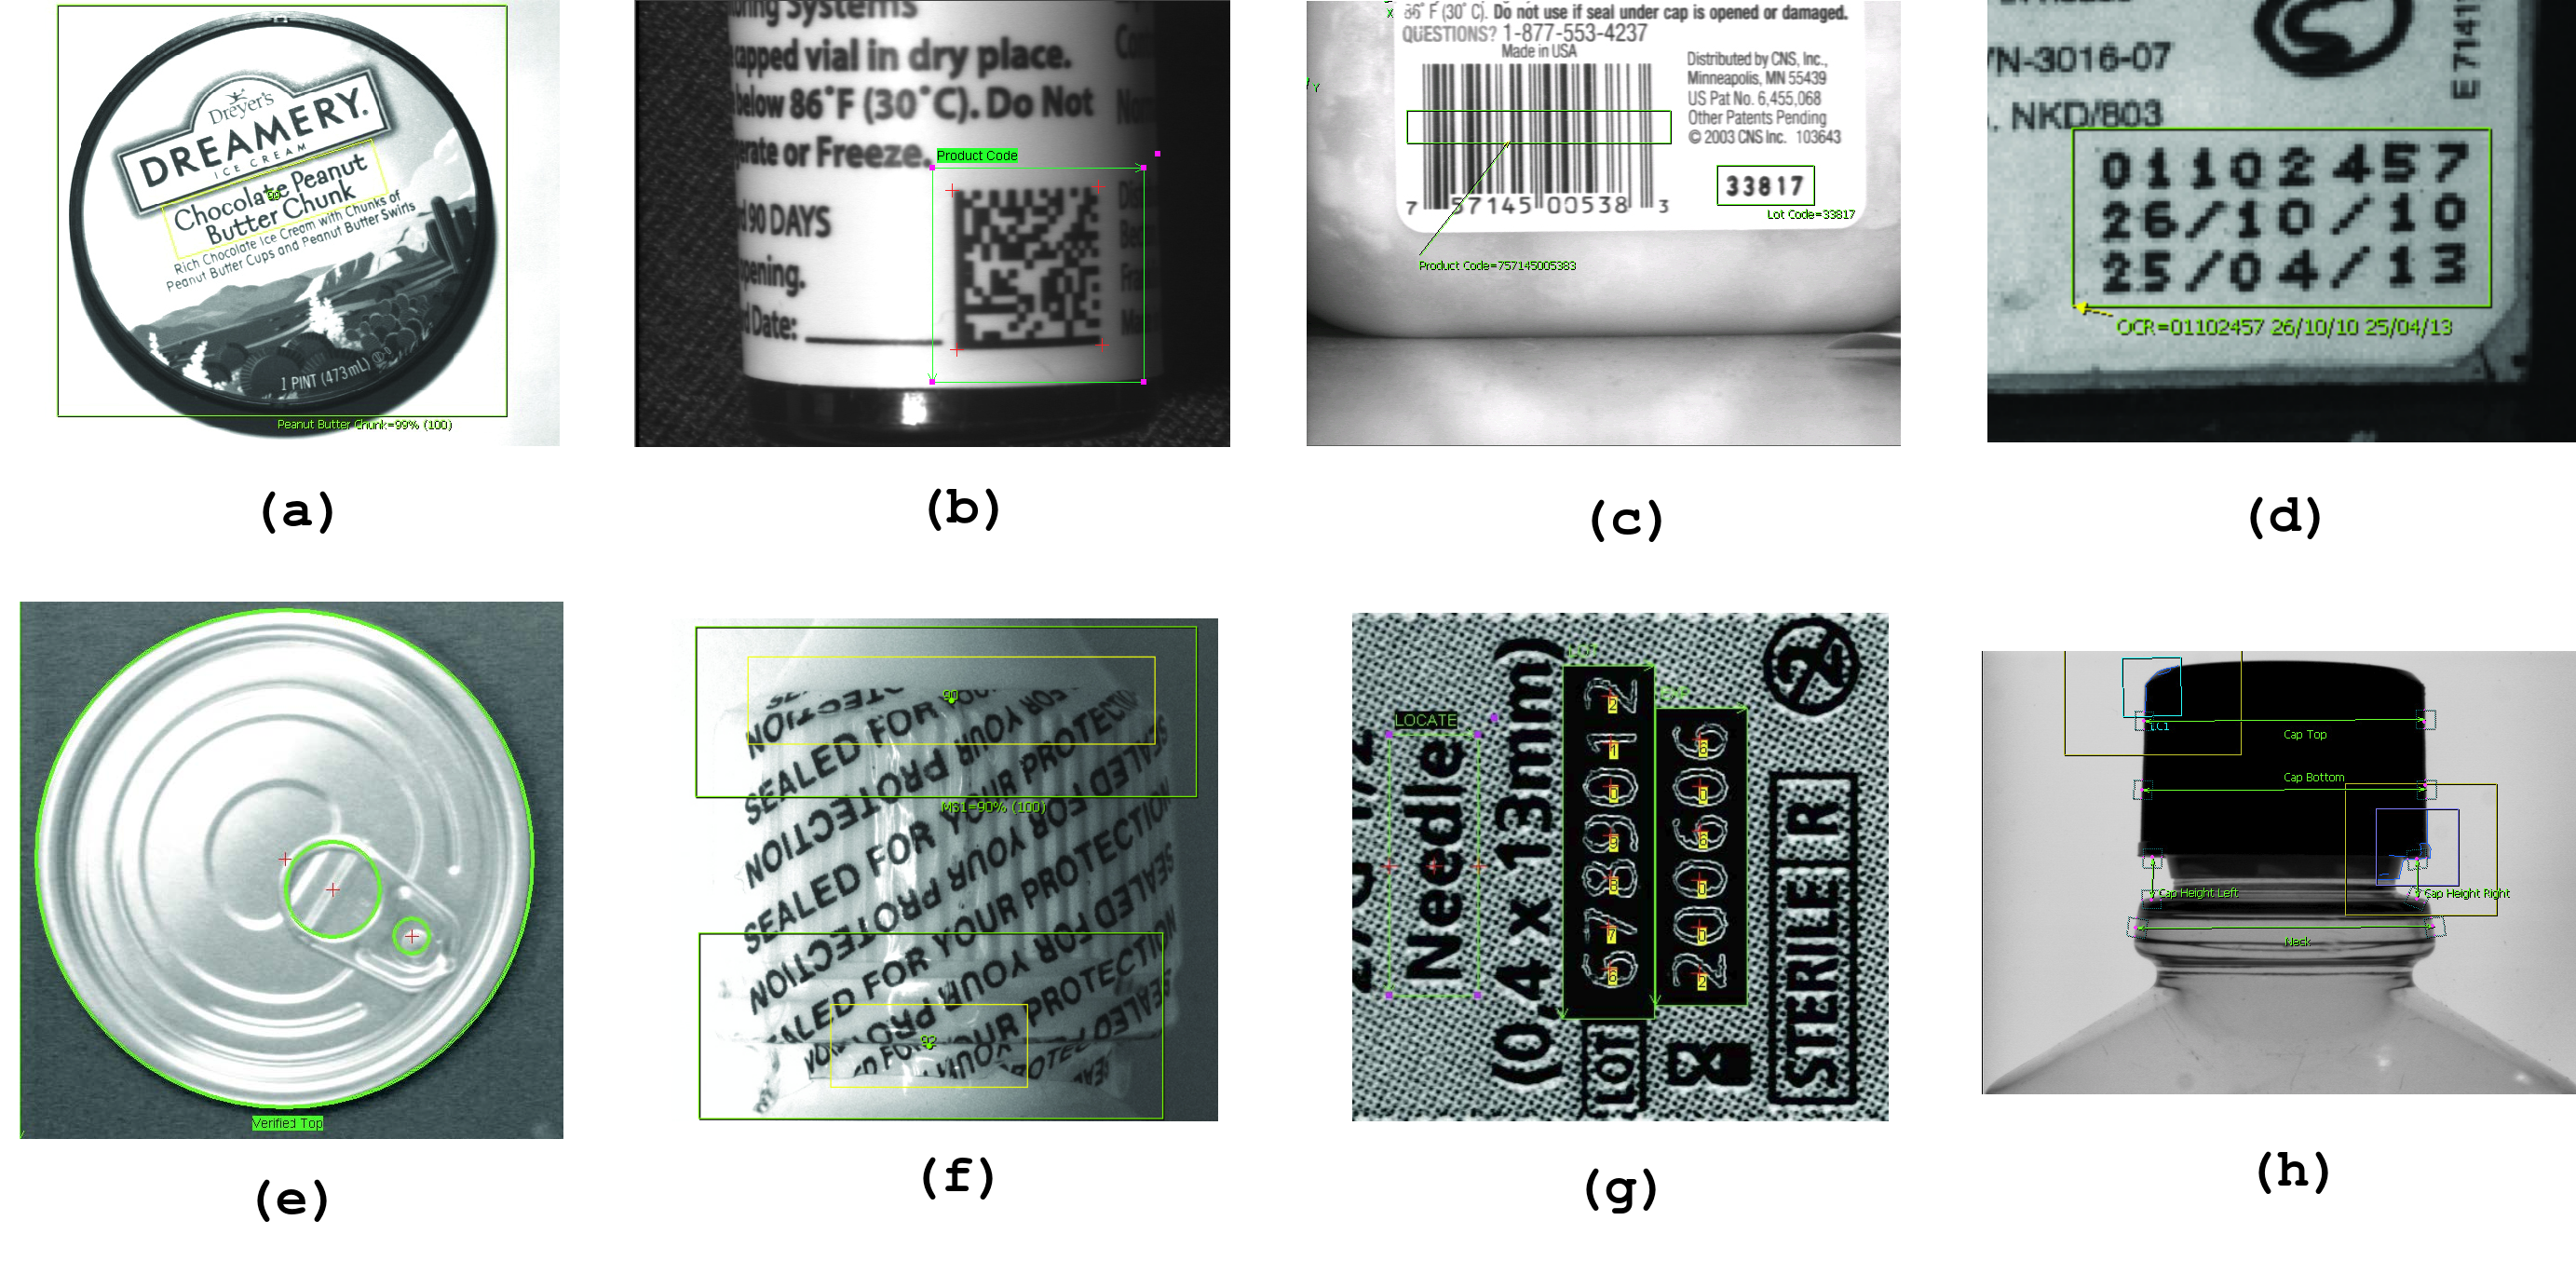
\includegraphics[scale=0.17]{Figures/industry.png}
\decoRule
\caption[Visión en la industria]{Presencia, aplicación e integridad de etiquetas (a), códigos 2D (b), códigos de barras (c), validación de lote, fecha y código (d), orientación de piezas montadas (e), correcto sellado (f), calidad de impresión (g), presencia y cierre de tapones (h). }
\label{fig:Industry}
\end{figure}

% Deportes
En los deportes quizás la aplicación más conocida sea el Ojo de Halcón (Figura~\ref{fig:Ojohalcon}), que se utiliza en los torneos de tenis de alto nivel para determinar la trayectoria de la pelota y saber si entró o no en el campo contrario. Además la visión artificial se usa en numerosos deportes sobretodo en estudios estadísticos post-partido para averiguar el tiempo de posesión del balón en los partidos de fútbol o los kilómetros recorridos por cada jugador en el terreno de juego, entre muchos otros.

\begin{figure}[th]
\centering
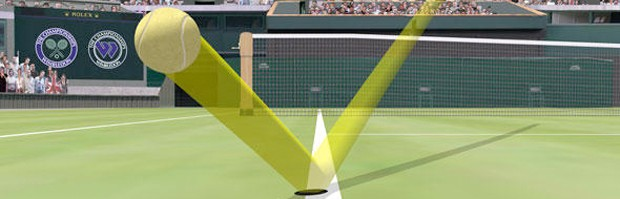
\includegraphics[scale=0.6]{Figures/ojohalcon.jpg}
\decoRule
\caption[Ojo de halcón]{Ojo de Halcón en tenis}
\label{fig:Ojohalcon}
\end{figure}

Actualmente se pueden encontrar sistemas de asistencia y seguridad en los vehículos más modernos como; sistemas de frenado automático de emergencia, asistente de mantenimiento de carril o aparcado automático. Aunque estos sistemas se entienden como asistentes o ayudas a la condución, el conductor sigue tomando la gran responsabilidad de la navegación.

La empresa israelí \textbf{Mobileye}\footnote{https://www.mobileye.com/} presentará su primer modelo de vehículo completamente autónomo, junto a Intel y BMW, en 2021. El cerebro de la máquina se basa en un sensor, que identifica lo que ocurre a su alrededor al instante: los carriles, las señales de tráfico, otros automóviles, motos, bicicletas e incluso a los peatones. En la Figura~\ref{fig:Car} se puede ver una captura de la vista del coche antes de parar en un semáforo.

\begin{figure}[th]
\centering
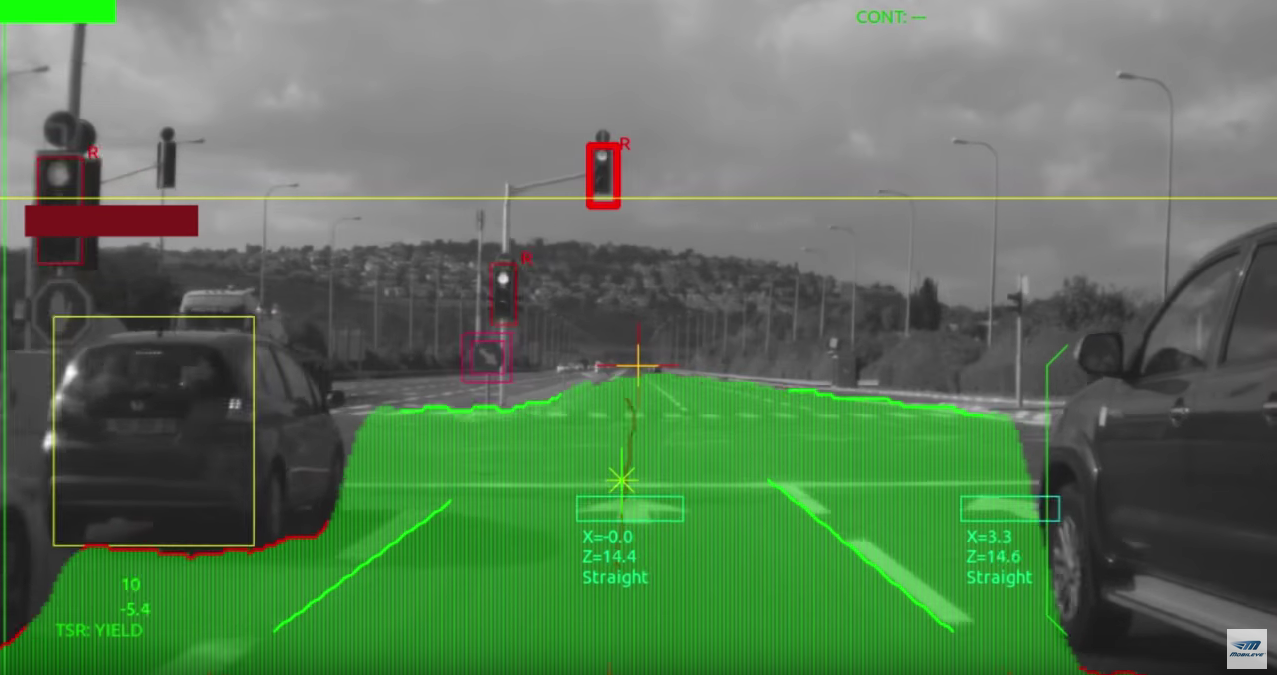
\includegraphics[scale=0.3]{Figures/car.png}
\decoRule
\caption[Visión para la autoconducción]{Vista del coche antes de parar en un semáforo.}
\label{fig:Car}
\end{figure}


\section{Autolocalización visual}
Dentro de la visión artificial se encuentra la autolocalización visual consiste en conocer la localización 3D de la cámara en todo momento solamente con las imágenes capturadas y sin disponer de ninguna información extra. Debido al gran abanico de posibilidades que abre resolver este problema, se sitúa en uno de los retos más importantes dentro del campo de la robótica.

%coches
Esta técnica se plantea en los sistemas de navegación automáticos naúticos, terrestres y aéreos. Actualmente numerosas empresas están invirtiendo en este tipo de sistemas en el que apuestan por una navegación total o parcialmente autónoma.

La autolocalización visual es una técnica que permite aplicaciones de realidad aumentada, que es el término que se usa para definir una visión directa o indirecta de un entorno físico del mundo real, cuyos elementos se combinan con elementos virtuales generados por ordenador para la creación de una realidad mixta en tiempo real.

Aunque se ha popularizado con el juego de \textbf{Pokémon Go}\footnote{http://www.pokemongo.com/es-es/}, cada vez son más los gigantes tecnológicos que se interesan por ella. La empresa sueca Ikea ya cuenta con una aplicación móvil que permite ver su catálogo en realidad aumentada (Figura~\ref{fig:Ikea}).

\begin{figure}[th]
\centering
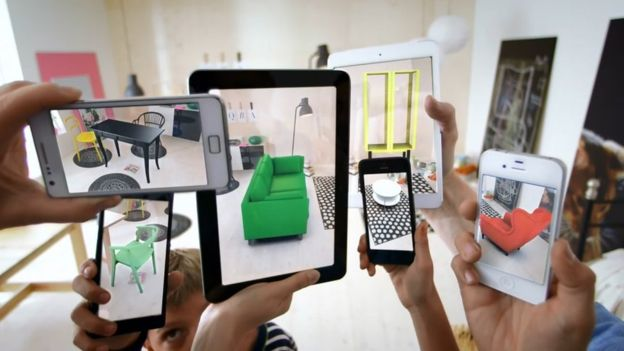
\includegraphics[scale=0.7]{Figures/ikea.jpg}
\decoRule
\caption[Ikea con realidad aumentada]{Catálogo Ikea con realidad aumentada.}
\label{fig:Ikea}
\end{figure}

Puesto que la realidad virtual es una experiencia ficticia, tiene gran potencial en el mundo de los videojuegos. Pero no es el único. También puede tener aplicaciones en medicina, la industria del cine, la moda, los deportes o la publicidad.

%-----------------------------------
%	SECTION Técnicas de autolocalización
%-----------------------------------
%\section{Técnicas de autolocalización visual}

Las técnicas de autolocalización ha suscitado gran interés por los investigadores en los últimos años. El problema ha sido abordado por dos comunidades distintas, por un lado la de visión artificial que denominó al problema como \textbf{structure from motion (SfM)}, donde la información es procesada por lotes, capaz de representar un objeto 2D a 3D con solo unas cuantas imágenes desde diferentes puntos de vista. Y por otro lado la comunidad robótica denominó al problema \textbf{SLAM} (\textit{Simultaneous Localization and Mapping}) que trata de resolver el problema de una manera más compleja adaptando el funcionamiento de los sistemas en tiempo real.

%-----------------------------------
%	SUBSECTION Structure from Motion
%-----------------------------------
\subsection{Structure from Motion (SfM)}

Las técnicas SfM se analizan generalmente de forma \textit{offline}, las escenas se graban a través de un conjunto de imágenes y luego se procesan, lo que permite realizar optimizaciones para el cálculo de la trayectoria, como por ejemplo el ajuste de haces.

Existen aplicaciones comerciales que utilizan estas técnicas como es el caso de la aplicación PhotoTourism \parencite{Reference2} desarrollada por Microsoft. Que consiste en el cálculo de la posición 3D en la que fueron captadas las imágenes, por ejemplo de un monumento, para después extraer el modelo 3D con el que el usuario puede interactuar libremente (Figura~\ref{fig:Tourism}).

\begin{figure}[th]
\centering
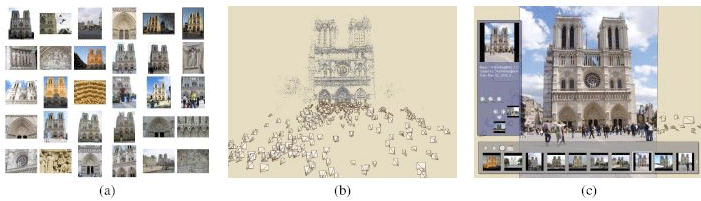
\includegraphics[scale=0.57]{Figures/phototourism.png}
\decoRule
\caption[PhotoTourism]{PhotoTourism: Se recogen una gran colección de imágenes (a), se reconstruyen los puntos 3D y los puntos de vista (b), por último la interfaz permite al usuario interactuar moviendose a través del espacio 3D mediante la transición entre fotografías.}
\label{fig:Tourism}
\end{figure}

%-----------------------------------
%	SUBSECTION Visual SLAM
%-----------------------------------
\subsection{Visual SLAM}

En el problema conocido como \textit{Simultaneous Localization and Mapping} (SLAM) busca resolver los problemas que plantea colocar un robot móvil en un entorno y una posición desconocidas, y que él mismo se encuentre capaz de construir incrementalmente un mapa de su entorno consistente y a la vez utilizar dicho mapa para determinar su propia localización.

La solución a este problema conseguiría hacer sistemas de robots completamente autónomos que junto con un mecanismo de navegación el sistema se encontrara con la capacidad para saber a dónde desplazarse, ser capaz de encontrar obstáculos y reaccionar ante ellos de manera inteligente.

La resolución al problema SLAM visual ha suscitado un gran interés en el campo de la robótica y se han propuesto muchas técnicas y algoritmos para dar solucón al problema, como es el caso del artículo de \cite{Reference1}. Y aunque algunas de ellas han obtenido buenos resultados en la práctica siguen surgiendo problemas a la hora de buscar el método más rápido o el que genere un mejor resultado con menos índice de fallo. La búsqueda de algoritmos y métodos que resuelvan completamente estos problemas sigue siendo una tarea pendiente.

Uno de los trabajos más importantes en el ámbito es el de monoSLAM de Davison\footnote{http://www.doc.ic.ac.uk/\textasciitilde ajd/} \parencite{Reference5} que propone resolver este problema con una única cámara RGB como sensor y realizar el mapeado y la localización simultáneamente. El algoritmo propuesto por Davison utiliza un filtro extendido de Kalman para estimar la posición y la orientación de la cámara, así como la posición de una serie de puntos en el espacio 3D. Para determinar la posición inicial de la cámara es necesario a priori dotar de información con la posición 3D de por lo menos 3 puntos. Después el algoritmo es capaz de situar la cámara en el espacio tridimensional y de generar nuevos puntos para crear el mapa y servir como apoyo a la propia localización de la cámara. En la Figura~\ref{fig:Monoslam} se pueden ver unas capturas de pantalla sobre uno de los experimientos realizados.

\begin{figure}[th]
\centering
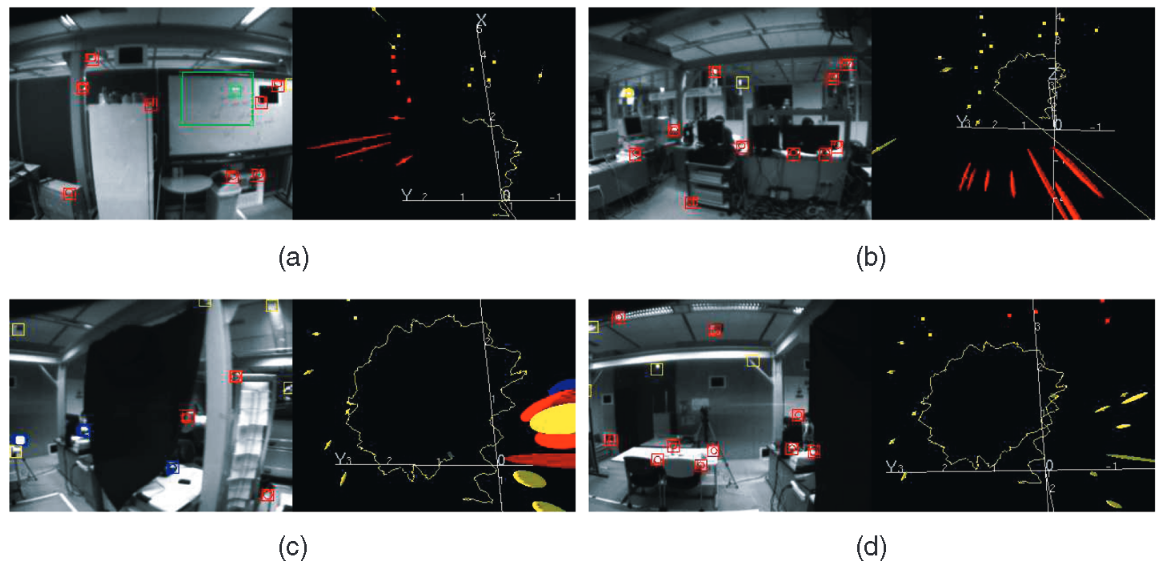
\includegraphics[scale=0.35]{Figures/monoslam.png}
\decoRule
\caption[MonoSLAM]{MonoSLAM: Un robot humanoide camina en una trayectoria circular de radio 0.75m. La estela amarilla muestra la trayectoria estimada del robot, y las elipses muestran los errores de localización.}
\label{fig:Monoslam}
\end{figure}

Es importante destacar también la trascendencia que ha tenido el trabajo PTAM \parencite{Reference6} que viene a solucionar uno de los principales problemas que tienen los algoritmos monoSLAM; el tiempo de cómputo, ya que aumenta exponencialmente con el número de puntos (Figura~\ref{fig:Ptam}). Para ello se aborda el problema separando el mapeado de la localización, de tal modo que solo la localización deba funcionar en tiempo real, dejando así que el mapeado trabaje de una manera asíncrona. Este algoritmo parte de la idea de que solo la localización es necesaria que funcione en tiempo real. PTAM hace uso de \textit{keyframes}, es decir, fotogramas clave que se utilizan tanto para la localización como para el mapeado y también de una técnica de optimización mediante ajuste de haces, como en SfM.

\begin{figure}[th]
\centering
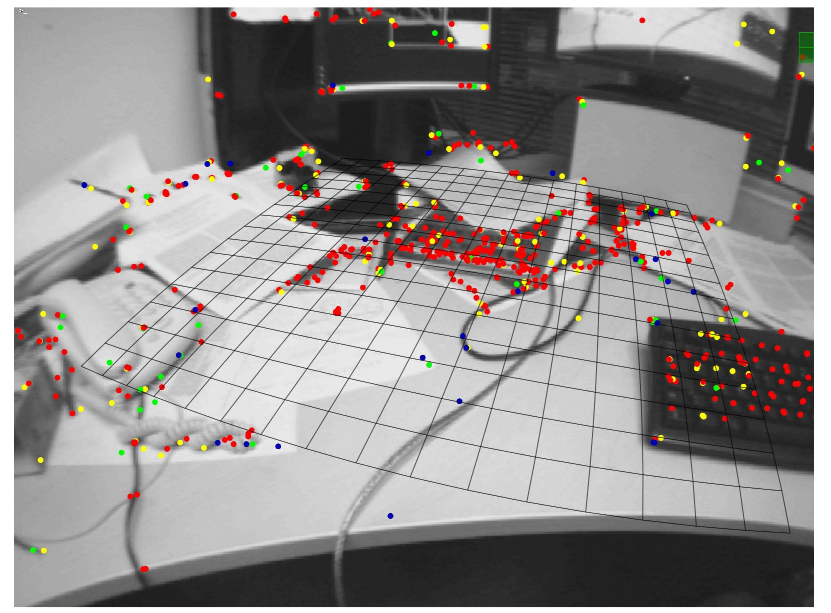
\includegraphics[scale=0.4]{Figures/ptam.png}
\decoRule
\caption[PTAM]{PTAM: Funcionamiento típico del sistema sobre un escritorio.}
\label{fig:Ptam}
\end{figure}

\subsection{Odometría visual}

Dentro de las familias de técnicas pertenecientes a Visual SLAM se encuentra la de odometría visual, que es la que abordaremos en este trabajo. Consiste en la estimación del movimiento 3D de la cámara en tiempo real. Es decir, el cálculo de la rotación y traslación de la cámara a partir de imágenes consecutivas. Se trata de una técnica incremental ya que se basa en la posición anterior para calcular la nueva.

En este tipo de algoritmos se suelen utilizar técnicas de extracción de puntos de interés, cálculos de descriptores y algoritmos para el emparejamiento. Normalmente el proceso es: una vez calculados los puntos emparejados se calcula la matriz fundamental o esencial y descomponerlas mediante SVD para obtener la matriz de rotación y traslación (RT) (\cite{Reference3}. \cite{Reference4}).

%-----------------------------------
%	SECTION Autolocalización visual en del Laboratorio de Robótica URJC
%-----------------------------------
\section{Autolocalización visual en el laboratorio de robótica URJC}

En esta sección se recapitulan algunos de los proyectos, dentro del campo de la autolocalización, realizados por compañeros en el laboratorio de robótica de la Universidad Rey Juan Carlos.

En el proyecto de Luis Miguel López Ramos \parencite{ref1} se diseña y programa un algoritmo que estima en tiempo real la posición y orientación de una cámara móvil autónoma en un entorno estático, utilizando exclusivamente las imágenes obtenidas por la cámara. El algoritmo se valida experimentalmente haciendo uso de una cámara de videoconferencia real y en condiciones de laboratorio.

Se calcula, por tanto, la trayectoria realizada y se muestra en una ventana de gráficos OpenGL junto con un modelo de la cámara y las regiones de confianza de los puntos de referencia. (Figura~\ref{fig:ramos}).

\begin{figure}[th]
\centering
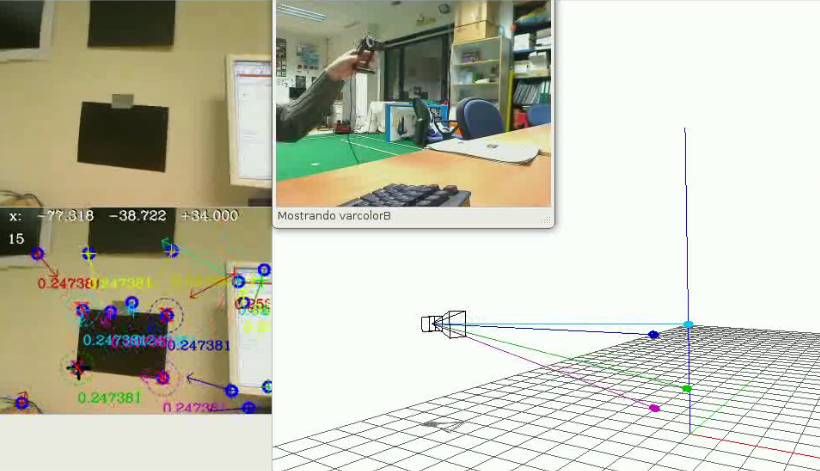
\includegraphics[scale=0.463]{Figures/cap-ramos.png}
\decoRule
\caption[Captura de pantalla, PFC de Luis Miguel]{Captura de pantalla del componente desarrollado por Luis Miguel.}
\label{fig:ramos}
\end{figure}

Eduardo Perdices García \parencite{ref3} propone en su trabajo de fin de master un proyecto de robótica autónoma. Dentro de este área se desarrolla la \textbf{RoboCup}, donde un grupo de robots autónomos deben jugar al fútbol de forma cooperativa variando su comportamiento en función de su posición en el campo, por lo que es muy importante que el robot conozca su posición en todo momento. A partir de los distintos sensores con los que cuenta el robot, como sensores de ultrasonido, sensores laser o cámaras, el robot tiene que estimar su posición en el mundo que le rodea.

En este proyecto se han desarrollado las técnicas necesarias para autolocalizar a un robot humanoide Nao\footnote{http://aliverobots.com/nao/} dentro de un campo de fútbol de la plataforma estándar de la RoboCup utilizando solo una cámara como sensor externo.

Alberto Lopéz-Cerón Pinilla \parencite{ref2} caracteriza un algoritmo de autolocalización visual basado en marcadores. Para ello, desarrolla un componente que a partir de la detección de balizas visuales en una imagen, estima la posición y la orientación de la cámara, mostrando el modelo de la cámara resultante en una ventana OpenGL.

El algoritmo se ha validado experimentalmente realizando estudios de precisión en dos ámbitos: por un lado el de entorno simulado de Gazebo, haciendo uso de un modelo robótico virtual con sus cámaras asociadas, y por otro en un entorno real con una cámara de videoconferencia (Figura~\ref{fig:ceron}).

\begin{figure}[th]
\centering
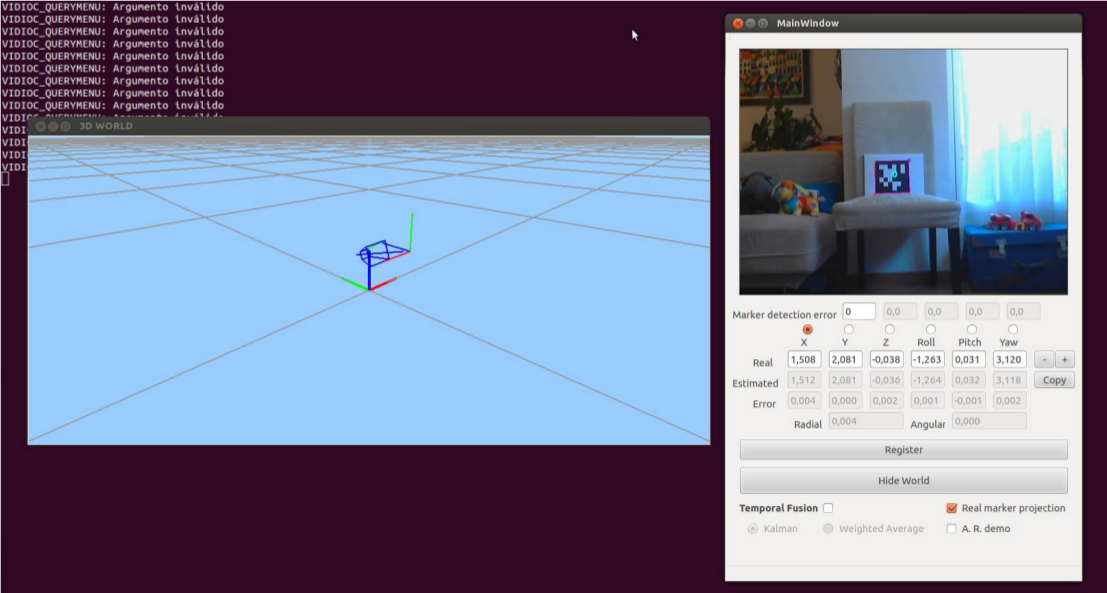
\includegraphics[scale=0.35]{Figures/cap-ceron.png}
\decoRule
\caption[Captura de pantalla, TFM de Alberto Lopéz-Cerón]{Captura de pantalla del componente desarrollado por Alberto Lopéz-Cerón.}
\label{fig:ceron}
\end{figure}

\newpage

En el proyecto fin de carrera de Daniel Martín Organista \parencite{ref5} se ha planteado un sistema de odometría visual, basado en sensores RGBD. El sistema desarrollado consta de algoritmos de estimación de la posición y trayectoria 3D de manera incremental en tiempo real, basándose en la información 3D ofrecida por el sensor RGBD. El sistema ha sido validado experimentalmente tanto en entornos reales como simulados (Figura~\ref{fig:dani}).

\begin{figure}[th]
\centering
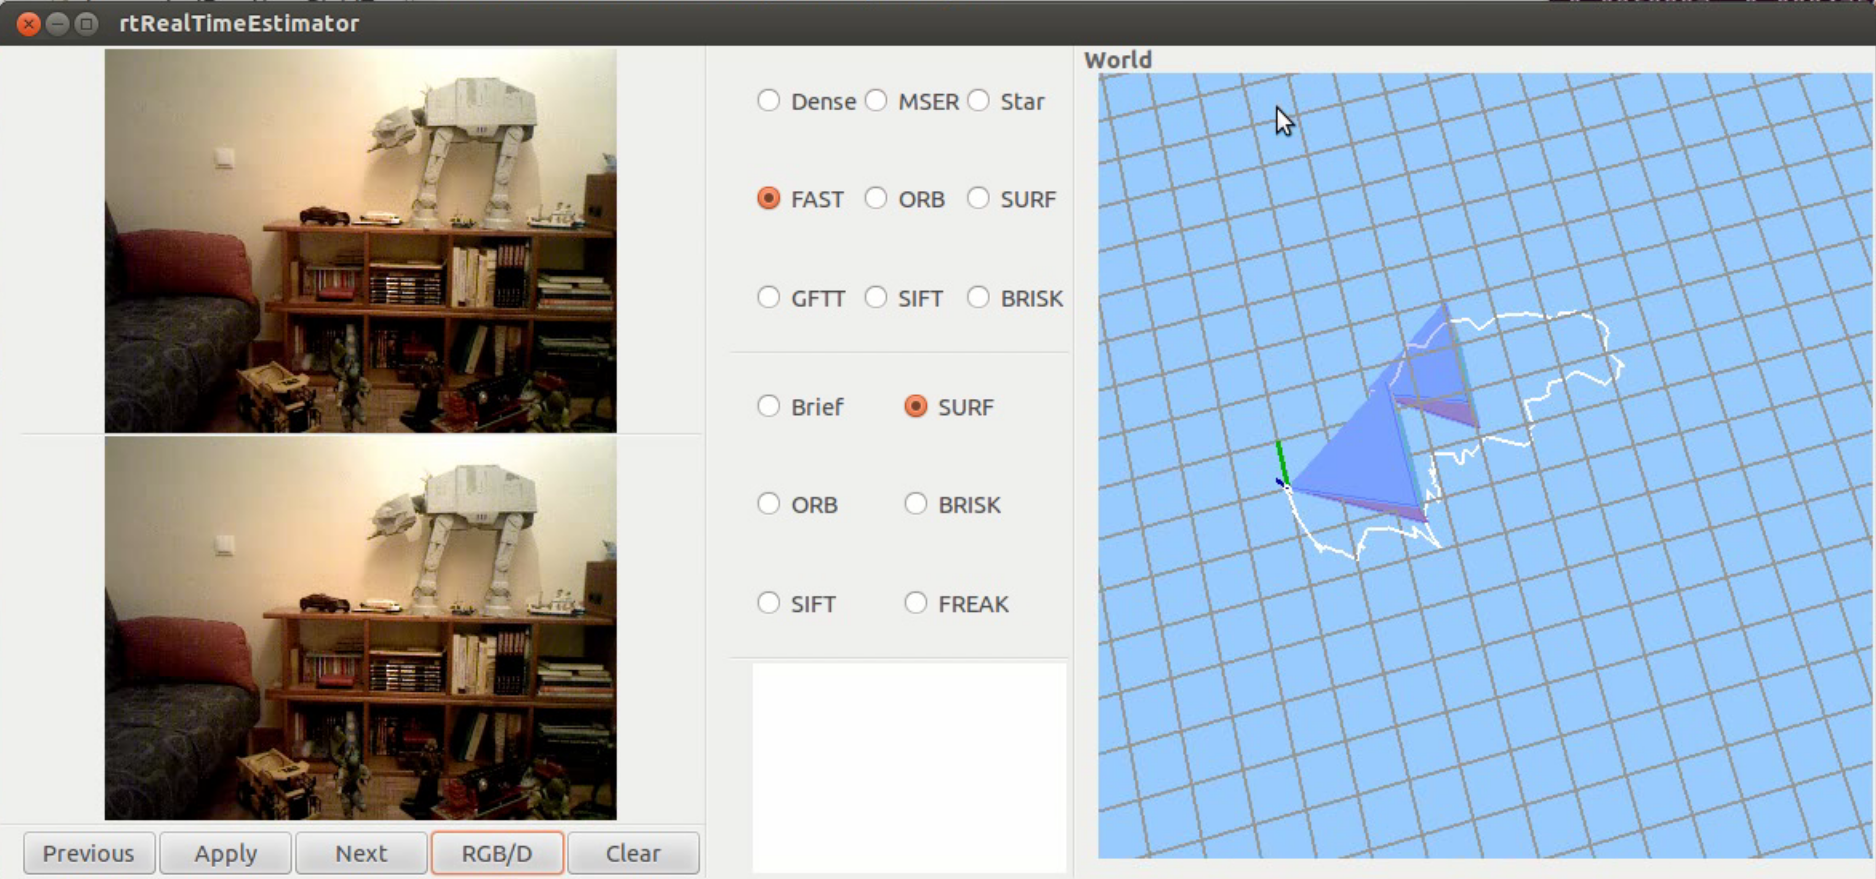
\includegraphics[scale=0.2]{Figures/cap-dani.png}
\decoRule
\caption[Captura de pantalla, PFC de Daniel Martín]{Captura de pantalla del componente desarrollado por Daniel Martín.}
\label{fig:dani}
\end{figure}

Por último, en el trabajo fin de master de Ignacio San Román Lana \parencite{ref4} se desarrolla un sistema clásico de odometría visual 3D en el que se emparejan puntos característicos entre fotogramas consecutivos o seguidos en el tiempo, para después optimizar un sistema de ecuaciones que estima la matriz fundamental. El resultado obtenido es mostrado en una ventana OpenGL en donde se puede ver la posición actual de la cámara y su recorrido.

El presente proyecto fin de carrera pretende unirse a los trabajos descritos en la búsqueda de algoritmos y técnicas de autolocalización visual, concretamente la odometría visual. En los próximos capítulos se detallará en la explicación de la solución adoptada.

El resto de la memoria consiste en 5 capítulos más:
\begin{itemize}
\item Objetivos - Se detallarán los objetivos del trabajo, así como la metodología llevada a cabo para la resolución del problema planteado.
\item Infraestructura - Se mostrarán las bases y técnologías empleadas.
\item Desarrollo - Se explicará el desarrollo del componente realizado y se detallarán tanto las bases teóricas como los algoritmos implementados.
\item Experimentos - Se muestran los experimentos realizados a fin de validar la solución optada.
\item Conclusiones - Se plantearán las conclusiones extraídas en base a los resultados obtenidos y se propondrán algunas líneas de trabajo futuras.

\end{itemize}
\chapter{Objetivos}

\label{Chapter2} % Change X to a consecutive number; for referencing this chapter elsewhere, use \ref{ChapterX}

Una vez presentado el contexto, en este capítulo se describen los objetivos concretos que se pretenden alcanzar. Tras una descripción del problema abordado y los requisitos, se detallará la metodología y la planificación que se ha llevado a cabo en la elaboración de este trabajo.

%------------------------------------------------
%	SECTION Descripción del problema
%------------------------------------------------
\section{Descripción del problema}

El objetivo principal de este trabajo es desarrollar un programa que solucione el problema de visualSLAM, para un sensor RGBD, a través de técnicas de odometría visual incrementales. El sistema debe ser capaz de averiguar la posición y orientación 3D de un sensor RGBD que se mueve libremente por el espacio y que va alimentando al sistema con las imágenes obtenidas en tiempo real.

Este objetivo principal se ha articulado en los siguientes cuatro subobjetivos:

\begin{enumerate}
 
\item \underline{Detección de puntos de interés}.
Creación de un módulo encargado de recoger de manera dinámica las imágenes RGB y DEPTH del sensor.

Desarrollo de un componente capaz de recoger, a través de diferentes técnicas, puntos de interés de una imágen con la opción de desarrollar algún filtro para añadir robustez a la detección.

\item \underline{Emparejamiento de puntos}.
Desarrollo del cálculo de correspondencias entre los puntos de interés en el fotograma actual y en el fotograma previo.

\item \underline{Estimación del movimiento 3D}.
Implementación de la matemática necesaria para una vez tenidos los puntos emparejados, entre dos fotogramas consecutivos, calcular la matriz de rotación y traslación (RT) que se necesitará para calcular en ese instante el movimiento incremental del sensor.

\item \underline{Pruebas y experimentos}.
El programa diseñado y construido se validará experimentalmente con un sensor real.

\end{enumerate}

Cada uno de los subobjetivos incluirán sus pruebas unitarias y su interfaz gráfico, desde donde se podrá analizar y verificar cada uno de los hitos.

%------------------------------------------------
%	SECTION Requisitos
%------------------------------------------------
\section{Requisitos}

A parte de las funcionalidades mencionadas en el apartado anterior, la solución final del proyecto debe satisfacer además los siguientes requisitos:

\begin{itemize}

\item Desarrollo del proyecto haciendo uso de la plataforma \textbf{JdeRobot 5.4.0}, que permite abstraerse de algunas de las funcionalidades de más bajo nivel como puede ser la captura de información del sensor o el protocolo de comunicaciones.

\item Como la mayoría de componentes de JdeRobot están en C++, el trabajo también se ha desarrollado utilizando el mismo lenguaje de programación.
%~\ref{ch:Chapter3}.

\item Debe funcionar bajo sistema operativo linux, en este caso Ubuntu 14.04 LTS.


\item Tiene que funcionar con un sensor RGBD real.

\end{itemize}


%------------------------------------------------
%	SECTION Metodología
%------------------------------------------------
\section{Metodología}

Para abordar un proyecto de tal envergadura es necesaria una metodología de desarrollo adecuada para ir progresando de una manera ordenada y efectiva. Se ha optado por el modelo en espiral basado en prototipos propuesto por B. Boehm en 1986 \parencite{Reference7}, ya que permite el desarrollo de una manera progresiva e incremental. 

Esta metodología permite el desarrollo de implementaciones parciales que van siendo probadas a medida que después de cada ciclo se va generando un prototipo más completo que el ciclo anterior. Por lo tanto, en cada ciclo o iteración se va añadiendo complejidad a la vez que se van generando funcionalidades nuevas.

Este modelo, utilizado en este trabajo, ha servido de gran ayuda, ya que permite ir avanzando de menos a más, con unos requisitos dependientes de los anteriores y a la vez diferentes para cada iteración. Además, permite ir evaluando y adaptando la evolución del desarrollo a nuestros intereses, algo que suele ocurrir normalmente en los proyectos de investigación.

En la Figura~\ref{fig:spiral} se puede observar el ciclo completo de desarrollo de software en el modelo en espiral. Cada etapa o ciclo completo está compuesto por cuatro fases:

\begin{itemize}
\item \underline{Identificación de objetivos}. En esta primera fase se deciden y se planifican los objetivos a alcanzar en la siguiente iteración partiendo de lo realizado en el ciclo anterior. En caso de la primera iteración se definen los objetivos iniciales.

\item \underline{Evaluación alternativa}. Aquí se definen requisitos y se estudian las distintas maneras de abordar los objetivos marcados de la etapa anterior. Se estudian los riesgos y se evaluan de qué manera se puedan reducir lo máximo posible. Se debe tener un prototipo antes de la siguiente etapa.

\item \underline{Desarrollo del producto}. En esta fase se diseña y se implementa el producto en base a lo planteado en las anteriores fases. Por último, se verifica y se prueba.

\item \underline{Planificación de la siguiente fase}. Considerando el resultado de la fase anterior, se planifica la siguiente considerando los errores cometidos y los resultados esperados, comenzando así una nueva iteración.

\end{itemize}

\begin{figure}[th]
\centering
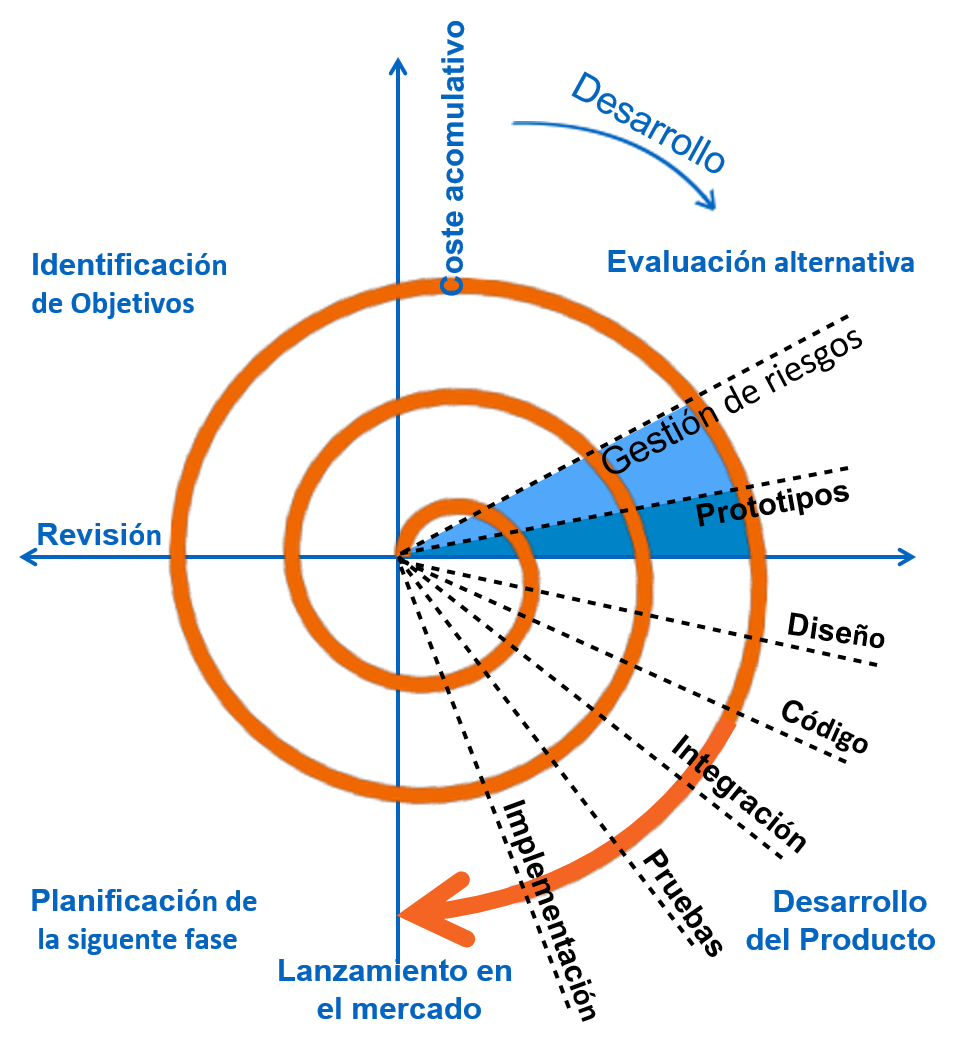
\includegraphics[scale=0.62]{Figures/spiral.png}
\decoRule
\caption[Ciclo de vida en espiral]{Ciclo de vida del desarrollo del \textit{software} en el modelo espiral.}
\label{fig:spiral}
\end{figure}

Para las fases de planificación y análisis se han mantenido reuniones semanales con el tutor, con intención de revisar, resolver problemas y encarar los nuevos objetivos establecidos.

A fin de documentar y guardar los hitos realizados en el desarrollo del proyecto, así como los errores cometidos y su posible solución, se ha llevado un seguimiento en mediawiki\footnote{http://jderobot.org/J.benitod-tfg} con los detalles de las diferentes iteraciones, ayudadas a veces por imágenes y/o vídeos.

Para la gestión de código se han usado herramientas \textit{software} de control de versiones, primeramente con Subversion (SVN)\footnote{http://svn.jderobot.org/users/j.benitod/pfc} y finalmente con GIT en un repositorio de GitHub\footnote{https://github.com/RoboticsURJC-students/2014-pfc-Javier-Benito}. Todo el código desarrollado es \textit{software} libre y está accesible a quien lo quiera.

%------------------------------------------------
%	SECTION Planificación
%------------------------------------------------
\section{Planificación del trabajo}

A lo largo del trabajo se han ido proponiendo etapas asesoradas y con supervisión del tutor. Las más importantes son:

\begin{enumerate}

\item \textbf{Familiarización de la herramienta JdeRobot}.

Esta etapa consistió en la instalación y el estudio de la plataforma, profundizando en el uso de algún componente con un objetivo muy concreto y sencillo.

Después, y para entender el funcionamiento de algunos de los componentes a bajo nivel más importantes para el trabajo, se propuso el desarrollo de algunos de ellos en otros lenguajes de programación tales como Java o Python.

\item \textbf{Aprendizaje de las herramientas específicas y técnicas de optimización}.

Aquí, a través de prácticas muy concretas se entendió el funcionamiento de algunas de las librerías esenciales para el proyecto.

\begin{itemize}

\item Se realizó un componente utilizando \textbf{PCL} para el cálculo de planos desde nubes de puntos.

\item Se utilizó \textbf{Eigen} para la resolución mediante optimización de sistemas sobredimensionados de ecuaciones, con descomposición QR y en valores singulares (SVD).

\item \textbf{GSL}, para la resolución de sistemas de ecuaciones, en este caso aplicado a un componente rectificador de imágenes.

\end{itemize}

\item \textbf{Creación de un componente para la extración de puntos de interés y emparejamiento}.

Aquí se empezó a desarrollar el componente final. Esta fase corresponde al desarrollo de la solución a los subobjetivos (1) y (2), en donde se comenzó por la extracción de puntos de interés con SIFT de las imágenes y los diferentes algoritmos para los emparejamientos.

\item \textbf{Registro entre dos nubes de puntos, relacionadas por una rotación, una traslación y ruido}.

En esta fase se propuso una práctica dedicada al subobjetivo (3) de estimación de movimiento incremental, en la que desde una nube de puntos y otra multiplicada por una matriz RT inventada, se sacaría a través de SVD dicha matriz a partir de las nubes de puntos iniciales y con la opción también de añadir ruido gaussiano a una de ellas.

\item \textbf{Integración y pruebas experimentales}.

Esta fue la etapa más larga y costosa. Surgieron multitud de errores que se tuvieron que ir depurando con cada iteración, proponiendo soluciones y alternativas. Fueron necesarias numerosas pruebas para conseguir un desarrollo capaz de aportar una solución estable.

\end{enumerate}
% Chapter Template

\chapter{Infraestructura} % Main chapter title

\label{Chapter3} % Change X to a consecutive number; for referencing this chapter elsewhere, use \ref{ChapterX}

En este capítulo se detallarán las herramientas base empleadas en la realización de este trabajo.

%----------------------------------------------------------------------------------------
%	SECTION Hardware
%----------------------------------------------------------------------------------------
%\section{Hardware}

%-----------------------------------
%	SUBSECTION Sensor
%-----------------------------------
\section{Sensores RGBD}

Los sensores RGBD son capaces de captar a parte de las componentes roja, verde y azul de la luz, información de profundidad (o "D"\ depth en inglés). Es decir, por cada píxel asocia la información de color con su correspondiente componente de profundidad. Esta tecnología fue desarrollada por la empresa israelí \textbf{PrimeSense}. El sensor Kinect dispone también de un micrófono multiarray con el cual puede predecir de dónde proviene el sonido.

En el 2010 Microsoft sacó al mercado el sensor Kinect (Figura~\ref{fig:Kinect}) para la consola de juegos Xbox 360 y Xbox One. Pronto se convirtió en uno de los dispositivos electrónicos más vendidos en todo el mundo después de su lanzamiento.

\begin{figure}[th]
\centering
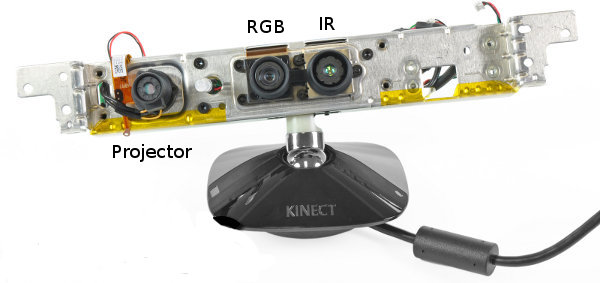
\includegraphics[scale=0.85]{Figures/ros_kinect.jpg}
\decoRule
\caption[Kinect sensor]{Sensor Microsoft Kinect}
\label{fig:Kinect}
\end{figure}

Este sensor salió al mercado a un precio mucho más reducido que algunos que existían antes que él por lo que el interés por este tipo de sensores se disparó y comenzaron a aparecen en diferentes áreas de la tecnología, como interfaces naturales de usuario (en inglés natural user interface, NUI), reconstrucción y realidad virtual o cartografía 3D.

El sensor utilizado en este trabajo es el \textbf{Asus Xtion PRO LIVE} que dispone de la misma tecnología comercializado por Asus, que proporciona profundidad, color y audio (utilizando un micrófono multiarray como el sensor Kinect). \footnote{https://www.asus.com/3D-Sensor/Xtion\_PRO\_LIVE/}

\begin{figure}[th]
\centering
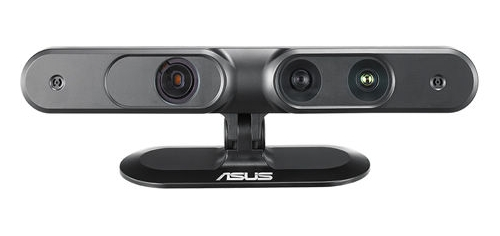
\includegraphics[scale=0.85]{Figures/xtion-pro-live.jpg}
\decoRule
\caption[Kinect sensor]{Asus Xtion PRO LIVE}
\label{fig:Kinect}
\end{figure}


\begin{table}
\caption{Especificaciones técnicas del Asus Xtion PRO LIVE}
\label{tab:xtion}
\centering
\begin{tabular}{ l | l }
\toprule
Campo de visión: & 58º H, 45º V, 70º D\\
\hline
Distancia de uso: & Entre 0.8m y 3.5m\\
\hline
Tamaño de la imagen de profundidad: & VGA (640x480) : 30 fps \\
				& QVGA (320x240): 60 fps\\
\hline
Resolución: & SXGA (1280*1024) \\
\bottomrule
\end{tabular}
\end{table}

Las especificaciones técnicas de este sensor se encuentran recogidas en la tabla ~\ref{tab:xtion}
%----------------------------------------------------------------------------------------
%	SECTION Software
%----------------------------------------------------------------------------------------
%\section{Software}

%-----------------------------------
%	SUBSECTION JDeRobot
%-----------------------------------
\section{JDeRobot}

JDeRobot es un proyecto desarrollado por el grupo de robótica de la Universidad Rey Juan Carlos \footnote{http://jderobot.org}. Consiste en una plataforma de desarrollo de aplicaciones robóticas y de visión artificial. Está en su mayoría escrito en C++, donde disponen de una colección de componentes capaces de comunicarse a través de ICE middleware \footnote{https://zeroc.com/products/ice}, los componentes pueden ejecutarse en diferentes ordenadores y pueden ser programados en diferentes lenguajes.

JdeRobot incluye numerosas herramientas, drivers, interfaces, librerías y tipos. Es \textit{software} libre con licencia GPL y LGPL. También utiliza \textit{software} de terceros como Gazebo, ROS, OpenGL, GTK y Eigen entre otros.

La versión de JdeRobot empleada ha sido la versión 5.4.0. A continuación se detallarán los componentes de JdeRobot que han sido de utilidad para la realización de este proyecto.

\subsection{Biblioteca Progeo}

Es una biblioteca de geometría proyectiva incluida en JdeRobot, que proporciona funciones muy útiles que relacionan puntos en dos y tres dimensiones.

Ha sido realmente útil en este trabajo para que a partir de puntos en dos dimensiones (píxeles) y su correspondiente información de profundidad (distancia), sacar los puntos relativos de la cámara en tres dimensiones.

Progeo usa el modelo de cámara \textbf{Pinhole}, en la Figura~\ref{fig:Pinhole} se puede observar la representación geométrica de la retroproyección y la proyección. Este modelo es definido por unos parámetros intrínsecos y extrínsecos que definen la composición de todos los parámetros iniciales de configuración de la cámara. Los parámetros extrínsecos que establecen la posición 3D, foco de atención (foa) y roll, mientras que los parámetros intrínsecos determinan la distancia focal y el centro óptico o píxel central.

\begin{figure}[th]
\centering
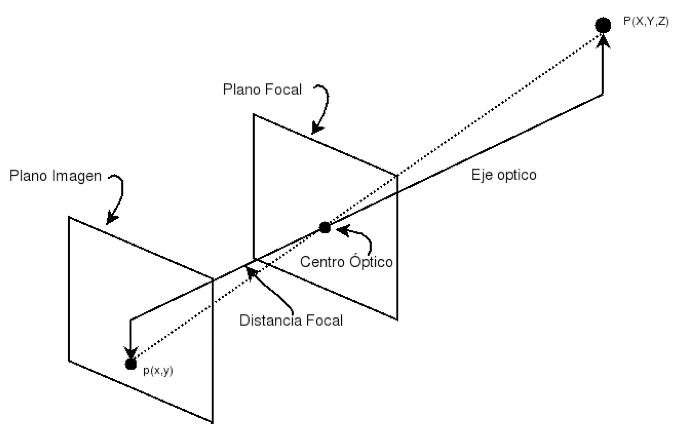
\includegraphics[scale=0.5]{Figures/pinhole-model.jpg}
\decoRule
\caption[pinhole]{Modelo de cámara Pinhole}
\label{fig:Pinhole}
\end{figure}

Las funciones que proporciona esta biblioteca son las siguientes:

\begin{itemize}
\item \textbf{Project}: Esta función permite proyectar un punto 3D del mundo al correspondiente pixel en 2D de la imagen de la cámara. 

\item \textbf{Backproject}: Esta función es capaz de a partir de las coordenadas de un píxel en 2D, obtener la línea de proyección que conecta la cámara y el foco con el rayo 3D que proyecta dicho píxel en el plano imagen. Con esto y conociendo la distancia real del punto 3D a calcular, se calcula las coordenas reales del punto 3D.

\item \textbf{DisplayLine}: Esta función permite conocer si una línea definida por dos puntos en 2D es visible dentro del plano imagen. 

\item \textbf{Display\_info}: Esta función muestra toda la información sobre la cámara utilizada.

\end{itemize}

\subsection{Biblioteca parallelIce}

Es otra librería incluída en JdeRobot, que soluciona el problema de latencia de información proveniente de los diferentes drivers, evitando la espera y proviniendo de un acceso asíncrono a una copia en local de las interfaces con muy bajo tiempo de procesado.

\subsection{Servidor OpenniServer}

OpenniServer es un driver que se comporta como un servidor y es capaz de proporcionar con un sensor RGBD (Kinect o Xtion), imágenes de color, de profundidad o nubes de puntos que son enviados a través de la interfaz ICE a un puerto específico, donde se pueden escuchar los datos. Este driver es el que se necesita para el funcionamiento de este trabajo ya que es desde donde se recogen tanto las imagenes de color (RGB) como las de profundidad (Depth) para su posterior procesado.

\subsection{Herramienta RGBDViewer}

Es una herramienta que permite enseñar la información proveniente de los sensores RGBD con openniServer como forma de visualización de los datos; imágenes RGB, DEPTH o nubes de puntos.

El funcionamiento corresponde a un hilo de ejecución llamado Control que se encarga de recolectar las imágenes provenientes del driver, una clase Shared para guardar y recoger los datos, y por último una clase Gui que se encargará de coger los datos (imágenes y nubes de puntos) guardados en Shared y mostrarlas.

%\begin{figure}[th]
%\centering
%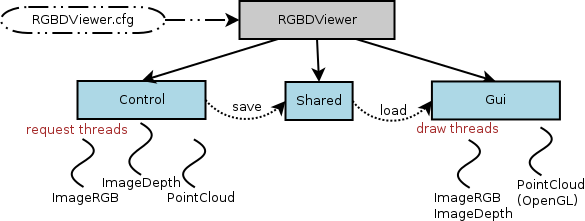
\includegraphics[scale=0.65]{Figures/rgbdviewer.png}
%\decoRule
%\caption[rgbdviewer]{Estructura del funcionamiento de RGBDViewer.}
%\label{fig:RgbdViewer}
%\end{figure}

Esta herramienta a servido como referencia para la realización de este trabajo. En la Figura~\ref{fig:RgbdViewer} podemos ver una captura de pantalla con las diferentes visualizaciones. 

\begin{figure}[th]
\centering
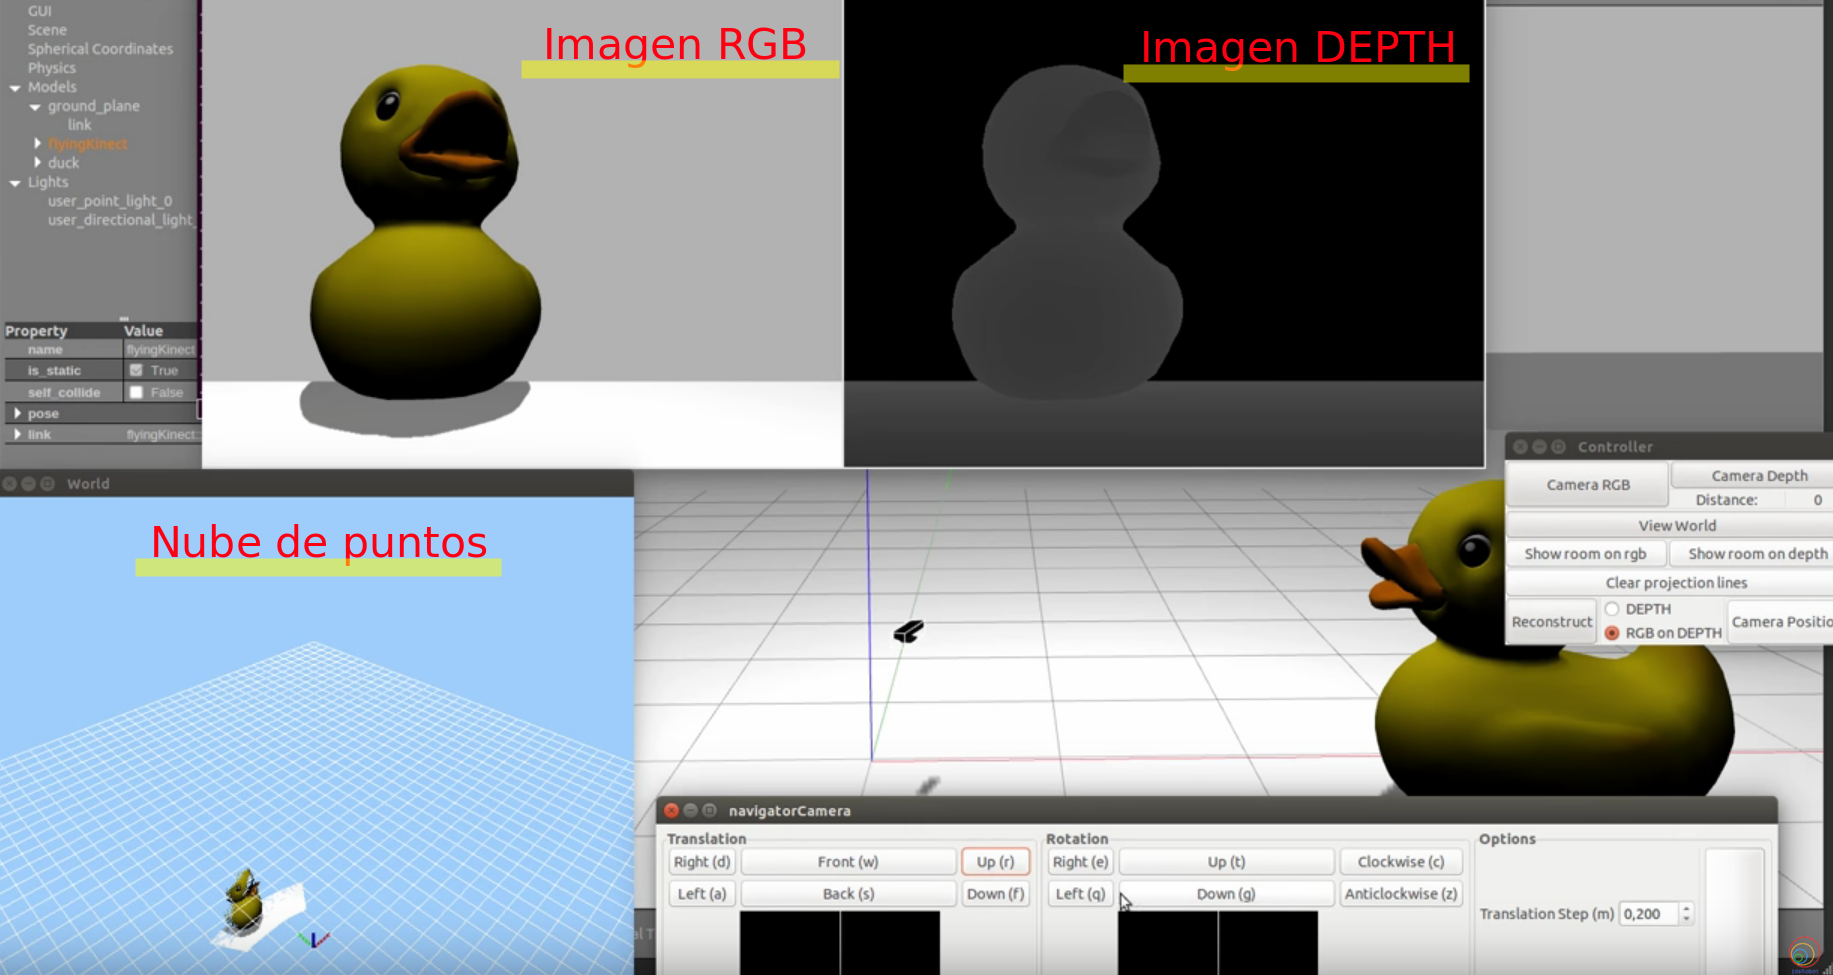
\includegraphics[scale=0.2]{Figures/rgbdviewer2.png}
\decoRule
\caption[rgbdviewer2]{Captura de pantalla del con las tres vistas de los diferentes datos, imagen de color, de profundidad y nube de puntos.}
\label{fig:RgbdViewer}
\end{figure}

\subsection{Pose3D}

Es una interfaz que define una posición en tres dimensiones (x, y, z, h) y una orientación con un cuaternión (q0, q1, q2, q3).

%\subsection{RGBPoint}

%Es una estructura de datos en la cual se pueden guardar puntos en tres dimensiones con coordenadas (x, y, z), color (r, g, b) y un identificador (id). 
%Para generar las nubes de puntos se ha usado un vector de esta estructura.

%-----------------------------------
%	SUBSECTION ICE
%-----------------------------------
\section{Biblioteca ICE de comunicaciones}

ICE (Internet Communications Engine) es un RPC framework desarrollado por ZeroC con soporte en C++, C\#, Java, JavaScript y Python entre otros. Se encuentra bajo doble licencia GNU GPL y código cerrado. Actúa como plataforma de comunicaciones y funciona bajo TCP/IP. \footnote{https://zeroc.com/products/ice}

En JdeRobot la podemos encontrar como librería y es utilizada como protocolo de comunicaciones entre los diferentes componentes de JdeRobot. En nuestro trabajo se ha usado la versión 3.5.1 y nos ha servido para establecer la comunicación entre el componente y el driver del sensor, recogiendo las imágenes de éste.

%-----------------------------------
%	SUBSECTION PCL
%-----------------------------------
\section{Biblioteca Point Cloud Library (PCL)}

PCL es una librería desarrollada en C++ para el procesamiento de imágenes 2D/3D y nubes de puntos. Está publicada con licencia BSD y libre bajo usos comerciales y de investicación. Está financialmente soportada por un consorcio de companías comerciales y su propia organización sin ánimo de lucro, \textbf{Open Perception}. A parte de los donadores y contribuidores individuales que aportan al proyecto. \footnote{http://pointclouds.org/}

Para simplificar el uso y el desarrollo, esta librería se encuentra dividida en módulos individuales de los que destacan el filtrado de puntos \textit{outliers} o de ruido, estructuras de datos, estimación 3D, algoritmos para la detección de puntos de interés, combinación, segmentación, algoritmos para el reconocimiento de objetos.
%En la Figura~\ref{fig:Grouping} se puede ver un ejemplo de reconicimiento de objetos basado en el módulo pcl\_recognition.

%\begin{figure}[th]
%\centering
%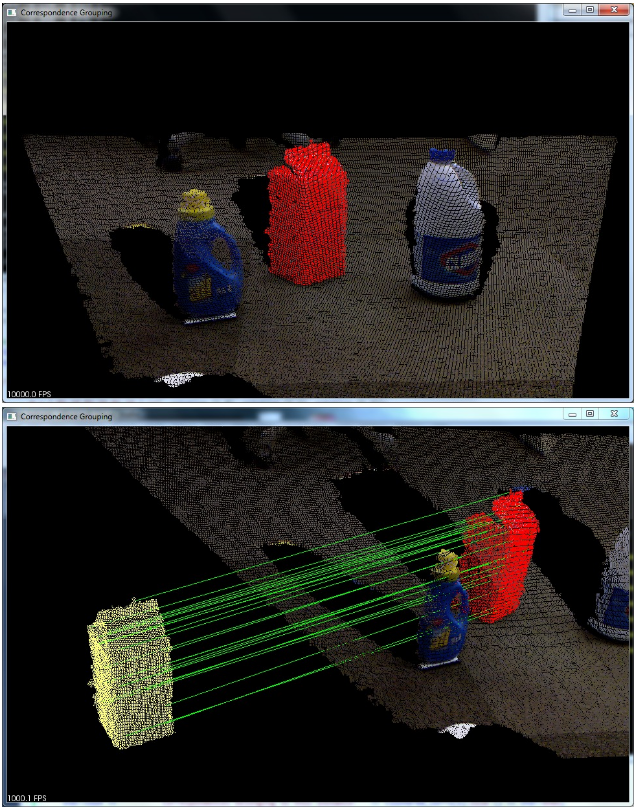
\includegraphics[scale=0.6]{Figures/correspondence_grouping.png}
%\decoRule
%\caption[grouping]{Reconocimiento de objeto 3D con PCL}
%\label{fig:Grouping}
%\end{figure}

En su página web disponen de mucha información y ejemplos prácticos que ayudan mucho a la compresión de todas las funcionalidades de esta librería. PCL también dispone de una librería i/o de entrada y salida para leer o crear nubes de puntos a partir de diferentes dispositivos, así como visualizadores 3D.


%-----------------------------------
%	SUBSECTION OpenCV
%-----------------------------------
\section{Biblioteca OpenCV}

OpenCV (Open Source Computer Vision Library) es una librería de código abierto que fue desarrollada para proporcionar una infraestructura común en aplicaciones de visión artificial y facilitar la inteligencia máquina, con mecanismos de aprendizaje y de interpretación de datos. Con licencia BSD da facilidades para su uso y su modificación bajo fines comerciales. \footnote{http://opencv.org/}

La librería contiene más de 2500 algoritmos. Estos algoritmos pueden ser usados para detectar y reconocer rostros, identificar objetos, clasificar acciones humanas determinadas en vídeos, seguimiento del movimiento de cámaras, seguimiento de objetos, extraer modelos de objetos 3D, producir nubes de puntos a partir de cámaras, encontrar imágenes similares de un conjunto, juntar trozos de imágenes para producir una imagen final con más resolución, etc... OpenCV tiene más de 47 miles de usuarios en la comunidad, excediendo los 14 millones de descargas, la librería es usada ampliamente en empresas, grupos de investigación y organismos gubernamentales.

OpenCV a sido diseñada de forma eficiente y con un fuerte enfoque en aplicaciones de tiempo real. Escrita en C/C++, la librería obtiene las ventajas del procesamiento multi-núcleo. Dispone de interfaces en C++, C, Python, Java y MATLAB y es soportada por diferentes sistemas operativos como Windows, Linux, Android y Mac OS.

En este trabajo se ha utilizado la versión 2.4.8 y se ha usado a la hora de identificar puntos de interés y para los distintos métodos de emparejamiento. En la Figura~\ref{fig:SiftDetector} se puede apreciar un ejemplo de su uso en la detección de puntos de interés sobre un entorno real.

\begin{figure}[th]
\centering
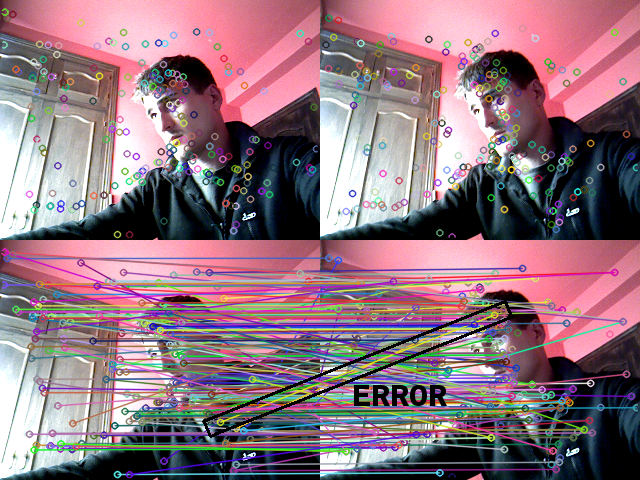
\includegraphics[scale=0.8]{Figures/sift-detector.png}
\decoRule
\caption[sift-detector]{Detección y emparejamiento de puntos de interés con OpenCV usando SIFT.}
\label{fig:SiftDetector}
\end{figure}

%-----------------------------------
%	SUBSECTION Eigen
%-----------------------------------
\section{Biblioteca Eigen}
Eigen es una librería de algebra lineal que permite hacer operaciones aritméticas con matrices y vectores, a través de los operadores comunes de C++, tales como +, -, * o a través de métodos especiales tales como dot(), cross(), etc... Para la clase \textit{Matrix} (matrices y vectores) los operadores solo soportan operaciones de álgebra lineal. En Figura~\ref{fig:Eigen} se puede ver un ejemplo de como de simple es hacer una multiplicación y una división por un escalar. \footnote{http://eigen.tuxfamily.org/}

\begin{figure}[th]
\centering
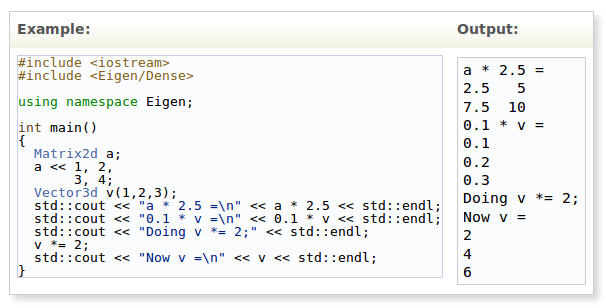
\includegraphics[scale=0.65]{Figures/eigen-multiplication.png}
\decoRule
\caption[eigen]{Ejemplo de una multiplicación y división por un escalar con Eigen.}
\label{fig:Eigen}
\end{figure}

Eigen es \textit{software} libre y desde la versión 3.1.1 tiene licencia MPL2 (LGPL3+ para las anteriores versiones). Se ha usado la versión 3.2.0 y ha sido de utilidad en este proyecto para realizar los cálculos de la matriz RT a través del los vectores de puntos 3D ya emparejados.

%-----------------------------------
%	SUBSECTION GTK
%-----------------------------------
\section{Biblioteca de interfaz gráfica GTK+}
GTK+, o the GIMP Toolkit es una herramienta multiplataforma de creación de interfaces gráficas. Es multiplataforma y está escrito en C, pero a sido diseñado para tener soporte para un gran rango de lenguajes, tales como Perl y Python. GTK++ tiene una gran colección de \textit{widgets} y interfaces para usar en la aplicación, tales como ventanas, botones, selectores, cajas de texto, etc.

La versión utilizada ha sido la 3.10.8. Es \textit{software} libre y parte del proyecto GNU. Con licencia LGPL, permite que sea utilizado por todos los desarrolladores, incluyendo aquellos que están desarrollando un  \textit{software} privativo. GTK+ ha sido utilizado en muchos proyectos y en grandes plataformas. \footnote{https://www.gtk.org/}

\subsection{Glade}
Glade es una \textit{RAD tool} (Rapid Application Development Tool) que permite desarrollar de manera fácil y rápida interfaces de usuario en GTK+ para el entorno de escritorio GNOME. La interfaz gráfica diseñada en Glade es guardada en un XML que usando los objetos GTK+ de \textbf{GtkBuilder} pueden ser cargados y utilizados por aplicaciones de forma dinámica como se ha hecho en este trabajo. \footnote{https://glade.gnome.org/}
%-----------------------------------
%	SUBSECTION OpenGL
%-----------------------------------
\section{OpenGL}
OpenGL es el principal entorno para el desarrollo de aplicaciones gráficas 2D y 3D interactivas. Desde 1992, OpenGL se ha convertido en la interfaz de aplicaciones gráficas más utilizada y soportada en la industria 2D y 3D, con miles de aplicaciones diponibles en diferentes plataformas. OpenGL ayuda al desarrollo de aplicaciones al incorporar un amplio conjunto de renderizado, mapeo de texturas, efectos especiales y otras potentes funciones de visualización. Se puede usar OpenGL en la mayoría de entornos de escritorio y diferentes plataformas. Es muy utilizada y conocida en la industria de los videojuegos.

Algunas de las ventajas de las que presume OpenGL son; que es un estándar de la industria, con soporte, multiplataforma y el único libre. Es estable, dispone de compatibilidad hacia atrás, escalable, fácil de usar y bien documentado. \footnote{https://www.opengl.org/}

Se ha usado la librería \textbf{Mesa 3D Graphics} en linux que es una implementación de la especificación de OpenGL con código abierto \footnote{https://www.mesa3d.org/}.

OpenGL en este trabajo se ha usado para visualizar la posición de la cámara, su estela y la colección de nubes de puntos obtenida y procesada de las imágenes RGB y de profundidad. En la Figura~\ref{fig:OpenGL} se puede apreciar una captura de pantalla con la posición de la cámara dibujada en el espacio tridimensional con el visualizador utilizado con OpenGL.

\begin{figure}[th]
\centering
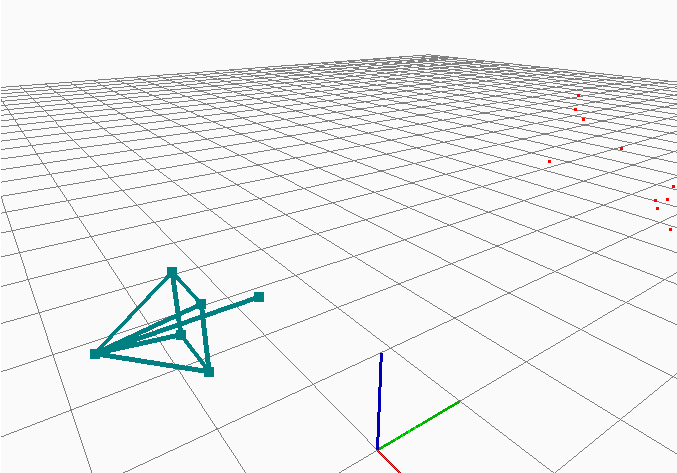
\includegraphics[scale=0.65]{Figures/camera-opengl.png}
\decoRule
\caption[opengl]{Captura de la posición de la cámara en el visualizador 3D con OpenGL.}
\label{fig:OpenGL}
\end{figure}
%% Chapter Template

\chapter{Desarrollo}

\label{Chapter4} % Change X to a consecutive number; for referencing this chapter elsewhere, use \ref{ChapterX}

Una vez presentado el contexto, los objetivos, así como las herramientas empleadas y los fundamentos teóricos, en este capítulo se detallará la solución software final desarrollada. Primero se presenta el diseño global utilizado y después se analizará en detalle el componente en cuestión realizado con una visión profunda del desarrollo por bloques y su funcionamiento.


%-----------------------------------
%	SECTION Diseño
%-----------------------------------
\section{Diseño}

El trabajo se basa principalmente en dos componentes; un componente de JDeRobot (\textbf{OpenniServer}) que funciona como driver del sensor y proporciona las imágenes obtenidas por éste y el componente realizado (\textbf{RealRTEstimator}) que se encargará, una vez recogidas las imágenes, de toda la lógica restante.

El objetivo del componente, como ya se ha comentado, consiste en analizar en tiempo real la posición y movimiento del sensor, por lo que el componente deberá dar una estimación en todo momento.

En la Figura~\ref{fig:diagram1} se puede apreciar el diagrama global de funcionamiento del componente desarrollado y su conexión con otros componentes para los diferentes datos de entrada.

\begin{figure}[th]
\centering
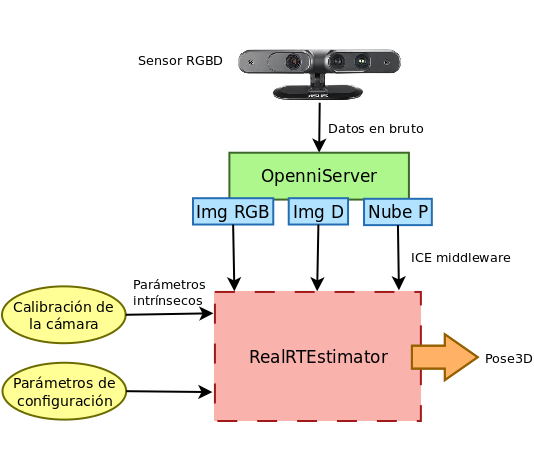
\includegraphics[scale=0.4]{Figures/diagram1.png}
\decoRule
\caption[Esquema general del componente RealRTEstimator]{Esquema global de funcionamiento.}
\label{fig:diagram1}
\end{figure}

OpenniServer se encarga de preparar y enviar las imágenes del sensor. El componente recoge las imágenes a través de ICE y éste es el encargado de procesarlas. También recibe los datos de los parámetros intrínsecos de la cámara así como algunos parámetros de configuración, como pueden ser la activación/desactivación de la interfaz de usuario o algunos parámetros configurables de algunos de los algoritmos internos. A su salida entrega una matriz RT que describe la posición y orientación absolutas en ese preciso instante de tiempo. 

Respecto al funcionamiento interno del componente se puede ver a grandes rasgos el diagrama en la Figura~\ref{fig:diagram2}. Se observa el diseño implementado así como sus bloques funcionales:

\begin{figure}[!ht]
\centering
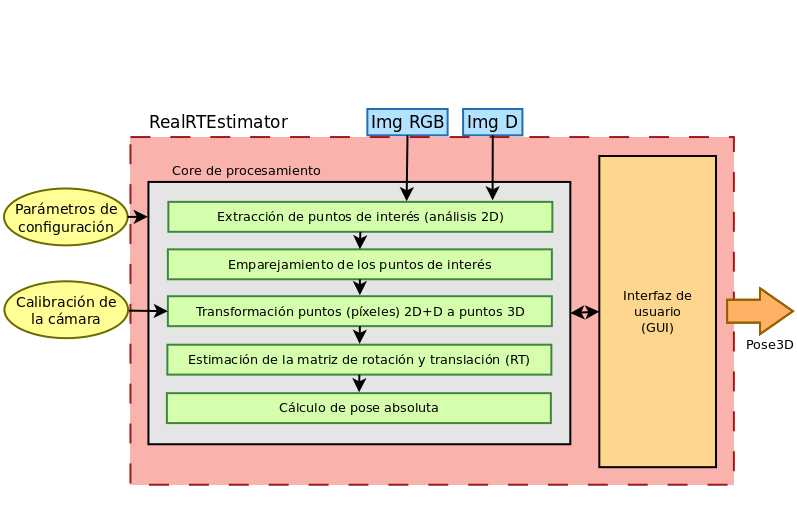
\includegraphics[scale=0.36]{Figures/diagram2.png}
\decoRule
\caption[Diagrama interno del componente RealRTEstimator]{Diagrama interno del componente RealRTEstimator.}
\label{fig:diagram2}
\end{figure}

\begin{itemize}
\item Extración de puntos de interés (análisis 2D) del fotograma actual.

\item Emparejamientos de puntos de interés en t con respecto a los puntos extraídos en el instante anterior (t-1).

\item Transformación de puntos (píxeles) en 2D más imagen de profundidad a nube de puntos en 3D.

\item Cálculo de movimiento. Es decir, estimación de la matriz de rotación y translación (Matriz RT).

\item Calculo de pose 3D absoluta.

\end{itemize}

En las siguientes secciones desglosaremos el funcionamiento de estos diferentes bloques funcionales.

%-----------------------------------
%	SECTION Extracción de características de una imágen
%-----------------------------------
\section{Análisis 2D}

El primer bloque del componente RealRTEstimator es el de análisis 2D. A partir de dos imágenes; la imagen de color y la de profundidad, se procede a la extracción de puntos de interés.

\subsection{Detección de puntos de interés}

El término puntos de interés o detección de características (\textit{Feature Detection} en inglés) hace referencia a la tarea de localizar en una imágen puntos relevantes o carácterísticos. Estos puntos suelen ser comunes y son fáciles de seguir de fotograma en fotograma.

Para entender cuales son estos puntos característicos podemos observar un ejemplo sencillo en la Figura~\ref{fig:feature_simple}. El cuadrado azul se encuentra en una área plana, y es difícil de seguir o encontrar. En cualquier lugar por donde se desplace parecerá que es el mismo. Para el cuadrado negro, que es un borde, igual para el desplazamiento lateral, sin embargo, para el desplazamiento vertical el punto ya cambia. Por último está el cuadrado rojo, que es una esquina. Para cualquier desplazamiento de esta figura, el punto ya es diferente, lo que significa que ese punto en la figura es único y por lo tanto vamos a poder identificarlo o seguirlo en diferentes imágenes. Así pues, las esquinas suelen ser candidatos idóneos para la detección puntos de carácterísticas en una imagen (en algunos casos las manchas también pueden ser consideradas buenas zonas).

\begin{figure}[!ht]
\centering
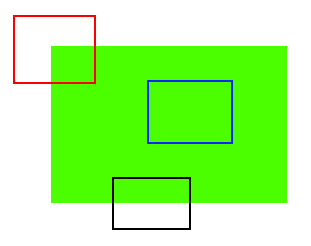
\includegraphics[scale=0.7]{Figures/feature_simple.png}
\decoRule
\caption[Ejemplo de puntos de interés]{Ejemplo sencillo de puntos característicos.}
\label{fig:feature_simple}
\end{figure}

Una vez entendido el concepto, el siguiente paso consiste, en averiguar cómo encontrar estos puntos de interés en una imagen real. Por ejemplo, una manera sencilla de hacerlo es buscar las regiones en las imágenes que contienen una gran variabilidad cuando son desplazadas (una pequeña distancia) hacia todas las direcciones de los alrededores.

Existen multitud de implementaciones para calcular estas carácterísticas en las imágenes. Uno de los primeros intentos en encontrar estas esquinas fue hecho por Chris Harris y Mike Stephens \parencite{Reference8}. El método, llamado \textit{Harris Corner Detector} transforma la simple idea a una fórmula matemática (\ref{eqn:Harris}) que básicamente encuentra la diferencia en intensidad por un desplazamiento (u,v) en todas las direcciones.

\begin{equation}
E(u,v)\,=\,\sum_{x,y}w(x,y)\,\,[I(x\,+\, u,\, y\,+\, v)-I(x,y)]^{2}
\label{eqn:Harris}
\end{equation}

Donde \textit{w(x,y)} es una ventana rectangular o gaussiana e I(x,y) corresponde a la intensidad. Aplicando algunos cálculos matemáticos que no vamos a entrar en detalle podemos llegar a la ecuación (\ref{eqn:Harris}) básica que determina si una ventana contiene una esquina o no.

\[ R=det(m)-k(trace(M))^{2} \]
\begin{equation}
R=\lambda_{1}\lambda_{2}-k(\lambda_{1}+\lambda_{2})^{2}
\label{eqn:Harris2}
\end{equation}

$\lambda_{1}$ y $\lambda_{2}$ son los autovalores de la matriz M, que determinarán si una región es esquina, borde o zona plana.

\begin{itemize}
\item Cuando $|R|$ es pequeño, que sucede cuando $\lambda_{1}$ y $\lambda_{2}$ son pequeños, la región es plana.

\item Cuando $R < 0$, que sucede cuando $\lambda_{1} >> \lambda_{2}$ o viceversa, la región es un borde.

\item Cuando $R$ es grande, que sucede cuando $\lambda_{1}$ y $\lambda_{2}$ son grandes y más o menos iguales, la sección es una esquina.

\end{itemize}

Más tarde, J. Shi y C. Tomasi hicieron una pequeña modificación que obtuvo mejores resultados comparados con los obtenidos en el detector de Harris \parencite{Reference9}. El resultado del detector \textit{Shi-Tomasi Corner Detector} se puede ver en la ecuación~(\ref{eqn:Shi})

\begin{equation}
R=min(\lambda_{1},\lambda_{2})
\label{eqn:Shi}
\end{equation}

Si $R$ es mayor que un determinado umbral, o dicho de otro modo; solo cuando $\lambda_{1}$ o $\lambda_{2}$ se encuentran por encima de un valor mínimo $\lambda_{min}$, se considera que cierta región es esquina. En la Figura~\ref{fig:shi_detector} se puede observar el resultado de aplicar dicho algoritmo en una imagen.

\begin{figure}[ht]
\centering
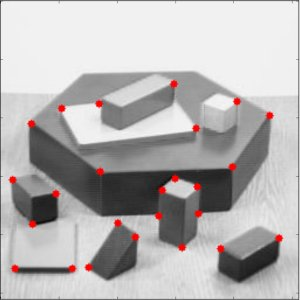
\includegraphics[scale=0.5]{Figures/shi-detector.jpg}
\decoRule
\caption[Ejemplo con \textit{Shi-Tomasi Corner Detector}]{Resultado de encontrar las mejores 25 esquinas de la imagen con \textit{Shi-Tomasi Corner Detector}.}
\label{fig:shi_detector}
\end{figure}

Existen varias implementataciones para el cálculo de carácterísticas de una imagen. A parte de las mencionadas, OpenCV proporciona entre otras \textbf{SIFT} y \textbf{SURF} que son las que hemos usado para el trabajo ya que permiten además de la detección de puntos de interés, el cálculo de descriptores.

\subsection{Cálculo de descriptores}

Una vez que se conoce el punto de interés, necesitamos asignarle una huella, algo carácterístico que nos permita encontrar el mismo en otra imagen. Para ello, se procede al cálculo de descriptores (\textit{Feature Description} en inglés).

Consiste en definir la región alrededor del punto de interés para poder buscar el punto con la misma región en otra imagen. Es decir, se guarda una descripción de la región del punto dado y se busca el mismo (o el que más se parezca) a otro punto perteneciente a otra imagen.

Una vez localizado el punto se podrá llevar un seguimiento de dónde está ese punto en otra imagen. No en todos los casos, se va a encontrar un descriptor perfecto para un cierto punto, por lo que al estudiar los emparejamientos se evaluará cuanto se parecen los despriptores entre sí. Esto lo veremos con detalle en la siguiente sección.

\subsubsection{SIFT}

SIFT (Scale-Invariant Feature Transform) soluciona uno de los problemas que se encontraban en los métodos anteriormente mencionados. Los métodos hasta ahora vistos para el cálculo de puntos de interés o esquinas, se suponen invariantes a la rotación, es decir, incluso si la images es rotada es posible encontrar las mismas esquinas. Esto es así porque una esquina sigue siendo una esquina si la imagen a sido rotada. Sin embargo, no contemplan los cambios de escala, un esquina no puede ser una esquina si la imagen ha sido escalada. En la Figura~\ref{fig:sift_scale_invariant} podemos ver un ejemplo de este hecho; una esquina en una pequeña imagen con una ventana no lo es cuando la imagen se amplia y se usa la misma ventana.

\begin{figure}[ht]
\centering
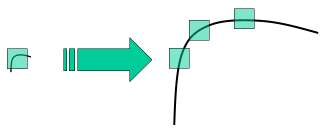
\includegraphics[scale=0.8]{Figures/sift_scale_invariant.jpg}
\decoRule
\caption[Ejemplo de sistema escalarmente variante]{Ejemplo de diferentes puntos con escala}
\label{fig:sift_scale_invariant}
\end{figure}

SIFT nace para proveer esta carencia de mano de D. Lowe \parencite{Reference10}. Un algoritmo escalarmente invariante que  localiza puntos de interés y calcula descriptores. Hay principalmente 4 etapas básicas en el algoritmo de SIFT:

\begin{enumerate}
\item \underline{Extrema detección en espacio-escala}

Para poder detectar características en diferentes escalas es necesario poder variar el tamaño de la ventana a ampliar. Para ello se utiliza un filtro de espacio-escala; un filtro LoG (Laplaciana de una Gaussiana) que con diferentes valores de $\sigma$ es capaz de detectar puntos de interés para diferentes escalas. $\sigma$ actúa como un parámetro de escala, para bajos niveles de $\sigma$ la gaussiana devuelve altos valores para las pequeñas esquinas, sin embargo, altos valores de $\sigma$ encajan bien para grandes esquinas.

Por lo tanto se busca a lo largo de la imagen y en diferentes escalas para encontrar el punto 

Así pues a lo largo de la imagen y en diferentes escalas tenemos una lista de $(x,y,\sigma)$ valores, donde $(x,y)$ representa el espacio y $\sigma$ la escala.

Sin embargo, el filtro LoG es muy costoso por lo que SIFT calcula una aproximación; la diferencia de gausianas con diferente $\sigma$ y el proceso se repetirá para diferentes octavas ($k\sigma$) como se puede apreciar en la Figura~\ref{fig:shif_dog}.

\begin{figure}[ht]
\centering
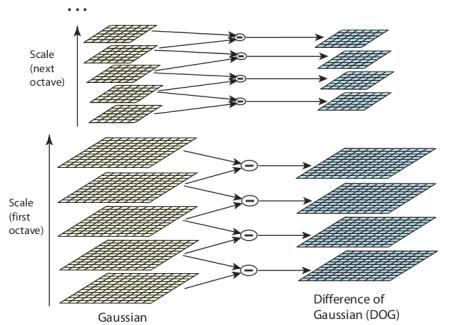
\includegraphics[scale=0.7]{Figures/sift_dog.jpg}
\decoRule
\caption[Diferencia de gaussianas en SIFT]{Proceso del cálculo de la diferencia de Gaussianas para diferentes octavas.}
\label{fig:shif_dog}
\end{figure}

Una vez obtenida la diferencia de gaussianas (DOG) se calcula el \textit{local-extrema}, por ejemplo, un píxel en una imagen es comparado con sus 8 vecinos y también con los 9 píxeles de la escala anterior y la posterior (Figura~\ref{fig:sift_local_extrema}).

\begin{figure}[ht]
\centering
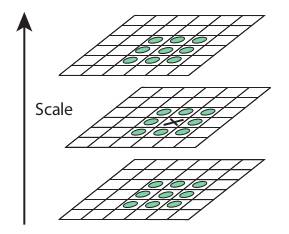
\includegraphics[scale=0.7]{Figures/sift_local_extrema.jpg}
\decoRule
\caption[Ejemplo de local-extrema en SIFT]{Ejemplo de local-extrema en SIFT.}
\label{fig:sift_local_extrema}
\end{figure}


\item \underline{Localización de puntos de interés}

Una vez que los puntos de interés se han localizado, se tienen que refinar a fin de obtener unos resultados más precisos. Por ello, se elimina cualquier punto de interés de bajo contraste, definido por el umbral \textit{contrastThreshold} y los puntos caracterizados como bordes por el umbral \textit{edgeThreshold}.

\item \underline{Asignación de orientación}

En este punto cada característica obtenida de la imagen se le asigna una orientación para mantener el algoritmo invariante ante la rotación. Se crean por tanto pntos característicos con la misma localización y escala pero en diferentes direcciones.

\item \underline{Descriptores}

Aquí el descriptor del punto es creado con una ventana 16X16 alrededor del punto.

\item \underline{Emparejamiento de puntos}

Los puntos de interés son emparejados en base a los vecinos. Se van seleccionando emparejamientos y cuando se encuentra un emparejamiento con menor distancia se selecciona. Los emparejamientos con una distancia mayor de 0.8 se eliminan.

\end{enumerate}

La implementación de SIFT en OpenCV es sencilla, partiendo de dos imagenes en escala de grises tenemos:

\begin{lstlisting}[style=CStyle]
	SiftDescriptorExtractor extractor;
 	SiftFeatureDetector detector;
 	std::vector<KeyPoint> keypoints_1, keypoints_2;

	// Keypoints detection
 	detector.detect( img_1, keypoints_1 );
 	detector.detect( img_2, keypoints_2 );
  	
 	// Descriptors calculation
 	extractor.compute(img_1, keypoints_1, descriptors_1);
 	extractor.compute(img_2, keypoints_2, >descriptors_2);
\end{lstlisting}

\subsubsection{SURF}

SURF (Speeded Up Robust Features) podría ser la evolución y versión rápida de SIFT. Desarrollada por Bay, H., Tuytelaars, T. y Van Gool, L. \parencite{Reference12} se introduce un nuevo algoritmo para la detección y cálculo de descriptores.

En vez de utilizar Laplaciana de la gaussiana (LoG) para encontrar el espacio de escala como SIFT. SURF va un poco más lejos y aproxima LoG con filtros de cuadros (\textit{Box Filter}). En la Figura~\ref{fig:surf1} se puede ver un ejemplo de tal aproximación.

\begin{figure}[ht]
\centering
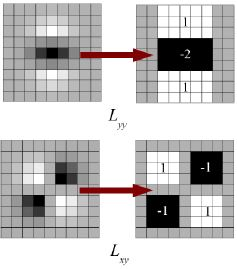
\includegraphics[scale=0.6]{Figures/surf-1.jpg}
\decoRule
\caption[Ejemplo de \textit{Box filter} en SURF]{Proceso con filtros de cuadros, \textit{Box filter}.}
\label{fig:surf1}
\end{figure}

La principal ventaja es que la convolución con cuadros es más fácil de cálcular con la ayuda de imagenes integrales. A parte, puede realizarse en paralelo para diferentes escalas.

Una vez calculado el escalado, se propone el cálculo de la orientación del punto de interés. Para obtener un punto invariante a las rotaciones, iluminación y orientación se utiliza \textit{wavelet de Haar} en la dirección $x$ e $y$ en una región circular de radio \textit{6s}\footnote{La \textit{s} hace referencia a un parámetro en el cómputo de descriptores de SURF que representa una escala que define los límites de las regiones circulares entorno al punto de interés.}. Después de haber evaluado las respuestas se busca la dirección predominante calculando la suma de todos los resultados dentro de una ventana con un ángulo de 60º. La región en la que se haya obtenido un mayor valor determinará la orientación buscada (Figura~\ref{fig:surf2}).

Para el cálculo del descriptor se construye una sección cuadrada en base a la orientación obtenida, alrededor del punto de interés y con un tamaño \textit{20s}x\textit{20s}. Esta región es dividida en sub-regiones de tamaño \textit{4s} x \textit{4s} y para cada una de ellas se calcula la respuesta de \textit{wavelet de Haar} de tamaño \textit{2s} tanto en $x$ como para $y$. Se genera el siguiente vector:

\begin{figure}[ht]
\centering
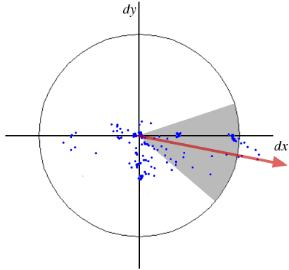
\includegraphics[scale=0.5]{Figures/surf-2.jpg}
\decoRule
\caption[Cálculo de orientación con SURF]{Cálculo de orientación con SURF.}
\label{fig:surf2}
\end{figure}

\begin{equation}
v=\left(\sum d_{x},\sum d_{y},\sum|d_{x}|,\sum|d_{y}|\right)
\end{equation}

Con el vector representado, para cada carácterística detectada el descriptor con SURF contendrá 64 dimensiones. A menor dimensión, mayor velocidad de cómputo y de emparejamiento, pero se consigue mayor distinción entre características. Para esto SURF tiene una versión extendida con 128 dimensiones.

En resumen, SURF añade un montón de mejoras para incrementar la velocidad en cada paso. Pruebas experimentales han demostrado que puede ser tres veces más rápido de SIFT. Aunque en robustez es comparable con SIFT, SURF se comporta bien en imágenes borrosas y con rotación pero no tanto cuando se cambian los puntos de vista o con una diferente condición de iluminación.

La implementación en código es similar a la de SIFT:

\begin{lstlisting}[style=CStyle]
	//-- Step 1: Detect the keypoints using SURF Detector
	int minHessian = 400;

	SurfFeatureDetector detector( minHessian );

	std::vector<KeyPoint> keypoints_1, keypoints_2;

	detector.detect( img_1, keypoints_1 );
	detector.detect( img_2, keypoints_2 );

	//-- Step 2: Calculate descriptors (feature vectors)
	SurfDescriptorExtractor extractor;

	Mat descriptors_1, descriptors_2;

	extractor.compute( img_1, keypoints_1, descriptors_1 );
	extractor.compute( img_2, keypoints_2, descriptors_2 );;
\end{lstlisting}



%-----------------------------------
%	SECTION Emparejamiento (\textit{matching})
%-----------------------------------
\section{Emparejamiento (\textit{matching})}

En esta sección abordaremos las distintas estrategias que se han implementado en el componente para el emparejamiento de puntos de interés. Los emparejamientos se harán por cada imagen/fotograma que llegue de la cámara después de la extración de puntos de interés.

El componente está recibiendo continuamente imágenes del sensor, por lo que el cálculo, al igual que la extración, se hará en cada iteración. Consiguiendo así una relación entre dos fotogramas consecutivos para analizar y posteriormente cálcular el desplazamiento sucedido. Estos emparejamientos nos darán margen para desechar algunos peores emparejamientos y filtrar por los mejores utilizando diferentes técnicas. Así pues, se intentará coger los mejores emparejamientos entre una imagen en $(t)$ y otra en $(t+1)$.

Se presentarán dos soluciones para este problema; una primera solución que calcula el emparejamiento de puntos mediante un mecanismo de \textbf{Fuerza Bruta} y en segundo lugar el uso de la librería \textbf{FLANN}, ambas proporcionadas por OpenCV.

\subsection{Fuerza Bruta}

El mecanismo de Fuerza Bruta es simple. Se coge el descriptor de una de las carácterísticas del primer fotograma (imagen en $(t)$) y se comprueba el parecido con todos los puntos de carácterísticas del segundo fotograma (imagen en $(t+1)$). Estos emparejamientos se evalúan a través de un parámetro de distancia. De todas las características, el descriptor que más se parezca al primero o el emparejamiento que tenga la menor distancia es el devuelto.

Para el cálculo de este emparejamiento se usará OpenCV. En primer lugar se tendrá que crear un objeto del tipo \textit{BruteForceMatcher} y pasarle como parámetro el tipo de medida para calcular la distancia, ya que depende del tipo de descriptor a utilizar.

Una vez creado el objeto dos métodos importantes son \textit{.match()} y \textit{.knnMatch()}. El primero devuelve el mejor emparejamiento. El segundo devuelve los $k$ mejores emparejamientos, donde $k$ es definido por el usuario.


El el siguiente ejemplo de código se puede observar como calcular los emparejamientos a través de OpenCV:

\begin{lstlisting}[style=CStyle]
	// matching descriptors
	BruteForceMatcher<L2<float> > matcher;
	vector<DMatch> matches;
	matcher.match(descriptors1, descriptors2, matches);
\end{lstlisting}

\textit{matches} por tanto será un array de objetos \textit{DMatch} (objeto de emparejamiento) con los siguientes atributos:

\begin{itemize}
\item \textit{DMatch.distance} - Parámetro de distancia entre descriptores. Cuanto menor distancia mejor emparejamiento.

\item \textit{DMatch.trainIdx} - Índice del descriptor de la segunda imagen con el resultado.

\item \textit{DMatch.queryIdx} - Índice del descriptor de la primera imagen a buscar.

\item \textit{DMatch.imgIdx} - Índice de la imagen resultado.
\end{itemize}

En Figura~\ref{fig:SiftDetector} podemos ver un ejemplo real de una prueba casera utilizando el algoritmo de Fuerza Bruta. Como se puede apreciar el tener que emparejar todos los puntos de una imagen al más parececido de la otra proporciona, incluso en una imagen muy parecida, errores que se van a tener que filtrar.

\begin{figure}[th]
\centering
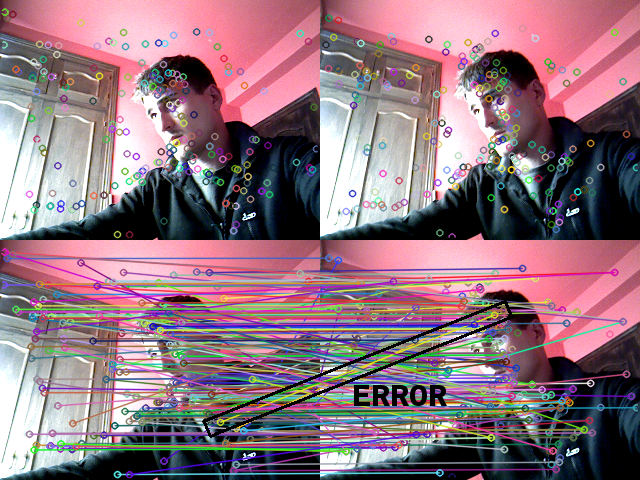
\includegraphics[scale=0.8]{Figures/sift-detector.png}
\decoRule
\caption[Captura real con SIFT]{Detección y emparejamiento de puntos de interés con OpenCV usando SIFT para el cálculo de puntos de interés y descriptores y Fuerza Bruta para el cálculo de los emparejamientos.}
\label{fig:SiftDetector}
\end{figure}



Por último, para la visualización OpenCV dispone del método \textit{.drawMatches()} que a partir de las dos imágenes y los emparejamientos obtenidos nos ayuda a dibujar los mismos para su visualización. Colocando las dos imágenes a tratar en horizontal y dibujando las líneas con los emparejamientos de una imágen a otra. En el caso de usar y querer visualizar los $k$ mejores emparejamientos existe también el método \textit{.drawMatchesKnn}.


\subsection{FLANN}

FLANN (Fast Library for Approximate Nearest Neighbors) es una librería que contiene una colección de algoritmos optimizados para encontrar emparejamientos.

Esta librería de OpenCV, es una implementación del trabajo de Marius Muja y David G. Lowe \parencite{Reference11}. Está pensada para trabajar con grandes conjuntos de datos y cuando los descriptores son representados por vectores de grandes dimensiones. Por lo que en estos entornos trabajará más rápido que el algoritmo de Fuerza Bruta.

FLANN provee de un sistema para elegir automáticamente el mejor algoritmo basado en la colección de datos. Dispone también de unos parámetros de entrada que permiten al usuario especificar la importancia de minimizar la memoria o el tiempo de compilación en lugar del tiempo de búsqueda.

La implementación en código con OpenCV es sencilla y muy parecida a la anterior:

\begin{lstlisting}[style=CStyle]
  //Matching descriptor vectors using FLANN matcher
  FlannBasedMatcher matcher;
  std::vector< DMatch > matches;
  matcher.match(descriptors_1, descriptors_2, matches);
\end{lstlisting}
\subsection{Resolución de errores}

Sobre el tema de filtrado de errores se han usado dos estrategias; se han cogido de todos los emparejamientos un porcentaje relativamente pequeño donde se encuentran los emparejamientos más acertados, tomando como medida de calidad la distancia ofrecida por los diferentes algoritmos y se ha incluido un filtro de sobresaliencia para el algoritmo de Fuerza Bruta.



\begin{itemize}
\item \underline{Mejores emparejamientos}. De $k$ emparejamientos obtenidos se ha implementado una función que ordena de menor a mayor la distancia de los emparejamientos obtenidos. Después y a través de la interfaz gráfica se podrá elegir el porcentaje de emparejamientos a emplear en la fase, que por defecto es un 20\%, es decir, $(k*0.2)$ puntos emparejados finales. Cuanto menor porcentaje mayor fiabilidad, pero menores resultados a pasar en la siguiente fase.

En la Figura~\ref{fig:bestPointsSift} se puede ver el resultado de aplicar este método tras un desplazamiento horizontal. Se comprueba que el número de fallos se reduce considerablemente.

\begin{figure}[th]
\centering
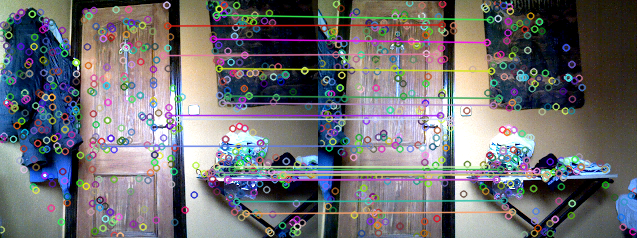
\includegraphics[scale=0.6]{Figures/best_points_sift.png}
\decoRule
\caption[Captura de los mejores puntos con SIFT]{Emparejamiento de los mejores X puntos ordenados por distancia.}
\label{fig:bestPointsSift}
\end{figure}

\item \underline{Filtro de sobresaliencia}. Este filtro surge de la necesidad de corregir un error común que se encontraba en los mejores emparejamientos por distancia. Existen ciertas situaciones en las que hay características de una imagen muy similares a otras de otra imagen y que corresponden a errores en el emparejamiento.

En la Figura~\ref{fig:similarCorrelation} se captura un ejemplo con dos de los mejores puntos medidos por distancia y se verifica que los dos mejores puntos se corresponden con el mismo punto en la imagen a buscar. Este error corresponde a una situación poco casual es origen de muchos errores en la estimación.

\begin{figure}[th]
\centering
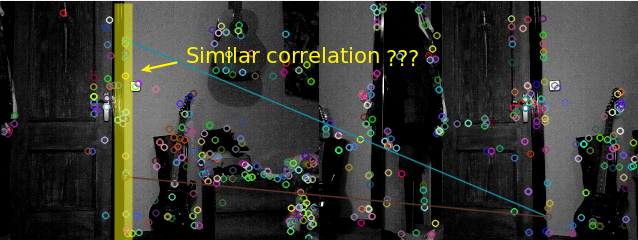
\includegraphics[scale=0.6]{Figures/similar-correlation.png}
\decoRule
\caption[Captura con error de los dos mejores puntos en SIFT]{Detección y emparejamiento de los mejores dos puntos.}
\label{fig:similarCorrelation}
\end{figure}

Se puede entender en la Figura~\ref{fig:similarCorrelation} que el punto con el resultado final del emparejamiento (imagen derecha) tiene a nivel de descriptores una mayor similitud que los demás, de ahí ese resultado. Se puede decir por tanto, que los dos mejores puntos tienen una correlación muy similar, al igual que tendrán los demás puntos a lo largo del marco de la puerta subrayado en amarillo.

Para ello, se ha empleado el método \textit{.knnMatch()} en el algoritmo de Fuerza Bruta que coge los $k$ mejores puntos. En este caso, se cogen los 2 mejores emparejamientos de todos los puntos y si la diferencia entre estos dos mejores emparejamientos es muy similar $(< 100)$ se desecha. Así pues, este filtro garantiza que el emparejamiento obtenido a través de los dos puntos es muy fuerte y no hay otro descriptor en la otra imagen con características similares.

El código para esta implementación es sencillo:

\begin{lstlisting}[style=CStyle]
	// Filtro de sobresaliencia
	vector<vector<DMatch> > matches_vector;
	matcher.knnMatch(descriptors1, descriptors2, matches_vector, 2);
	for (int i=0; i<matches_vector.size(); i++) {
		outNumber = matches_vector[i][1].distance - matches_vector[i][0].distance;
		if (outNumber >= OUTSTANDING_DISTANCE) {
			// Guardamos el emparejamiento
		}
	}
\end{lstlisting}

Donde \textit{OUTSTANDING\_DISTANCE} es el umbral mínimo de diferencia de distancias permitido, que por defecto se ha definido en 100.

Como diferencia, en esta ocasión como resultado del método \textit{.knnMatch()} se obtine un vector de vectores. Cada vector corresponde a un emparejamiento y por cada uno, otro vector con los $k$ mejores emparejamientos.

\end{itemize}

%-----------------------------------
%	SUBSECTION Obtención de puntos 3D
%-----------------------------------
\section{Obtención de puntos 3D}

Una vez obtenidos los puntos de interés y los mejores emparejamientos, se necesitará llevar a 3D los puntos calculados para el instante $(t)$\footnote{Como explicaremos más adelante, no se necesitarán calcular los puntos 3D para el instante $(t-1)$ ya que los puntos en ese instante ya se habrán calculado.}, para poder analizar en la siguiente fase el desplazamiento en tres dimensiones.

Esos puntos de interés en dos dimensiones, o mejor llamados; píxeles, se obtienen a partir de la imagen RGB que proviene del sensor, sin embargo, para este cálculo se necesitará además la imagen DEPTH correspondiente. O lo que es lo mismo, el mismo píxel o punto de la imagen a color debe corresponder con su homólogo en la imagen de profundidad. Se puede deducir que ambas imágenes deberán estar perfectamente sincronizadas para asegurarse de que ambas se corresponden con el mismo instante de tiempo. En la Figura~\ref{fig:diagramPoints3d} tenemos el diagrama de transformación de los puntos.

\begin{figure}[th]
\centering
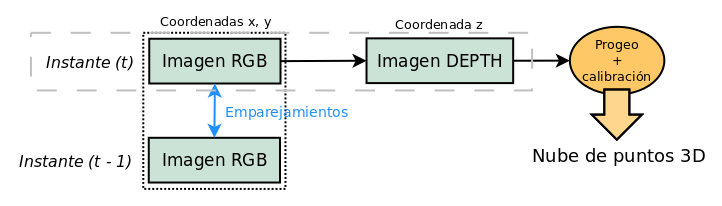
\includegraphics[scale=0.4]{Figures/diagram-points-3d.png}
\decoRule
\caption[Diagrama con la obtención de puntos 3D]{Diagrama de transformación a puntos 3D.}
\label{fig:diagramPoints3d}
\end{figure}

Para conseguir la información 3D se ha utilizado la librería de Progeo y su modelo de proyección \textit{PinHole}. Una vez obtenidos los puntos 2D más su información de distancia, se busca la recta de retroproyección correspondinete a cada uno de los píxeles de la imágen que se quieran transformar. Después se calcula el punto 3D, que será el que se encuentre a una distancia $d$ de la recta de retroproyección (ej: punto $P$ en la Figura~\ref{fig:camLine}).

\begin{figure}[th]
\centering
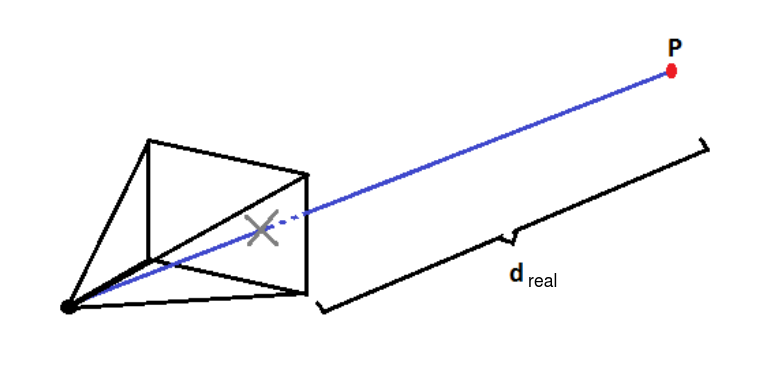
\includegraphics[scale=0.35]{Figures/cam-line.png}
\decoRule
\caption[cam-line]{Cálculo de punto 3D con la información de distancia $d$.}
\label{fig:camLine}
\end{figure}

La transformación de un píxel a su homólogo en 3D es compleja. El proceso de recostrucción está basado en un modelo proyectivo desde el centro óptico, por lo tanto, la distancia que se devuelve del sensor es la distancia perpendicular al plano imagen, y no la distancia real, tal y como se puede apreciar en la Figura~\ref{fig:distPoint}. Para ello, si se quiere calcular la posición 3D asociada a un píxel cuya recta de retroproyección es la que une el foco de la cámara y un punto BP (Figura~\ref{fig:calculate3d}) el punto que se quiere calcular no será el punto $P$, punto a una distancia $d$ del foco de la cámara y que nos da el sensor, sino el punto $Pr$ que corresponde al punto 3D real.

\begin{figure}[th]
\centering
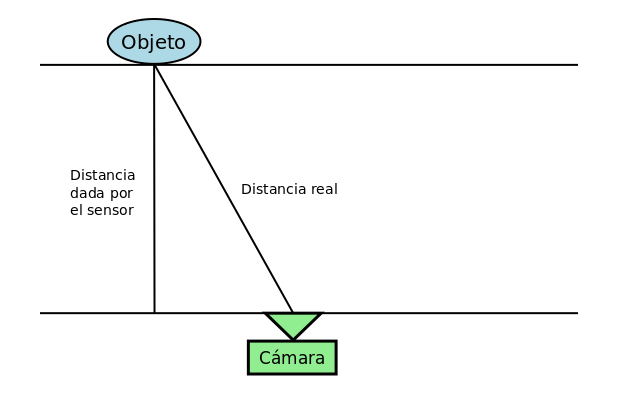
\includegraphics[scale=0.4]{Figures/dist-point.png}
\decoRule
\caption[dist-point]{Distancia real y la dada por el sensor.}
\label{fig:distPoint}
\end{figure}

Para calcular el punto $Pr$, se tiene que encontrar la intersección entre la recta de retroproyección y el plano $D$. Definimos el plano $D$ como el plano con vector normal $\vec{k}$ que pasa por el punto $Q$. El vector $\vec{k}$ se obtiene como vector unitario que une el centro óptico de la cámara con el foco de atención, $foa$ (\textit{focus of attention}). Este vector es un vector perpendicular al plano imagen. El $foa$ es un parámetro conocido que obtenemos en el proceso de calibración de la cámara junto con la orientación y el \textit{roll}\footnote{Movimento del sensor sobre el eje central del sensor, paralelo al $foa$ o foco de atención.} (parámetros extrínsecos). El proceso matemático es el siguiente:

\begin{figure}[th]
\centering
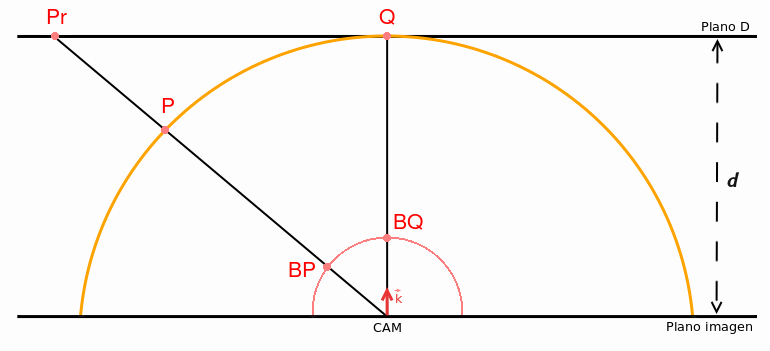
\includegraphics[scale=0.5]{Figures/calculate-3d.png}
\decoRule
\caption[calculate-3d]{Ejemplo de corrección de distancia.}
\label{fig:calculate3d}
\end{figure}

Se calcula el vector unitario $\vec{k}$ entre \textit{CAM} y $foa$:

\begin{equation}
\vec{k}=\frac{\overrightarrow{CAMFOA}}{|CAMFOA|}
\end{equation}

Una vez obtenido el vector $\vec{k}$ se obtiene el punto $Q$ que se encuentra a una distancia $d$ del sensor, con las ecuaciones paramétricas de la recta:

\begin{equation}
Q_{x}=CAM_{x}+d\cdot k_{x}
\end{equation}
\[ Q_{y}=CAM_{y}+d\cdot k_{y} \]
\[ Q_{z}=CAM_{z}+d\cdot k_{z} \]

Con esto se tendría el plano que contiene el punto $Pr$ que es el que se quiere calcular. Es decir, el punto sobre la recta que pasa por $BP$ a una distancia $D$ (distancia corregida) del punto \textit{CAM}.

Realizando los mismos cálculos, definimos el vector director de la recta \textit{CAMBP}; $\vec{v}$:

\begin{equation}
\vec{v}=\frac{\overrightarrow{CAMBP}}{|CAMBP|}
\end{equation}

Utilizando la ecuación paramétrica de la recta:

\begin{equation}
Pr_{x}=CAM_{x}+D\cdot v_{x}
\label{eqn:param}
\end{equation}
\[ Pr_{y}=CAM_{y}+D\cdot v_{y} \]
\[ Pr_{z}=CAM_{z}+D\cdot v_{z} \]


Como el punto $Pr$ se encuentra en el plano $D$, se tendrá que calcular la intersección de la recta recién calculada y el plano $D$. Para calcular el plano $D$ se aplica la ecuación del plano con los datos obtenidos; $Q$, $Pr$ y el vector normal al plano $\vec{k}$:

\begin{equation}
k_{x}(CAM_{x}+t\cdot v_{x}-Q_{x})+k_{y}(CAM_{y}+t\cdot v_{y}-Q_{y})+k_{z}(CAM_{z}+t\cdot v_{z}-Q_{z})=0
\end{equation}

Despejando $t$:

\begin{equation}
t=\frac{-k_{x}\cdot CAM_{x}+k_{x}\cdot Q_{x}-k_{y}\cdot CAM_{y}+k_{y}\cdot Q_{y}-k_{z}\cdot CAM_{z}+k_{z}\cdot Q_{z}}{k_{x}\cdot v_{x}+k_{y}\cdot v_{y}+k_{z}\cdot v_{z}}
\end{equation}

Por último, aplicando el resultado de $t$ sobre la ecuación~\ref{eqn:param} se obtiene el punto real buscado $Pr$.

%-----------------------------------
%	SUBSECTION Cálculo de movimiento
%-----------------------------------
\section{Cálculo de movimiento}

Una vez calculados los puntos 3D, el siguiente bloque del componente realizado es la estimación de movimiento. En este caso hay que calcular continuamente el movimiento relativo entre los instantes $(n-1)$ y $(n)$. Esto permite ir siguiendo la trayectoria y la orientación seguida por el sensor a lo largo del tiempo.

\subsection{Matriz RT}

La trayectoria seguida se definirá por una \textbf{matriz RT} (Rotación + Translación) 4x4 de la manera que muestra la Figura~\ref{fig:matrixRT}.

\begin{figure}[th]
\centering
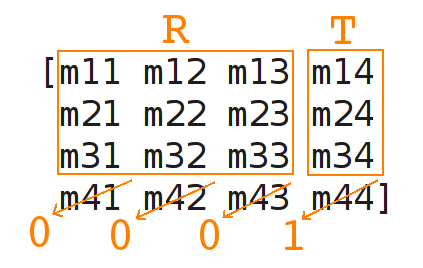
\includegraphics[scale=0.5]{Figures/matrixRT.png}
\decoRule
\caption[matrix-rt]{Matriz RT. Donde $R$ corresponde a la rotación y $T$ a la traslación.}
\label{fig:matrixRT}
\end{figure}

Donde cualquier rotación podrá ser expresada como combinación de tres rotaciones por cada eje:

\begin{equation}
R_{x}(\theta)=\left[\begin{array}{ccc}
1 & 0 & 0\\
0 & cos\theta & -sen\theta\\
0 & sen\theta & cos\theta
\end{array}\right]
\end{equation}
\begin{equation}
R_{y}(\theta)=\left[\begin{array}{ccc}
cos\theta & 0 & sen\theta\\
0 & 1 & 0\\
-sen\theta & 0 & cos\theta
\end{array}\right]
\end{equation}
\begin{equation}
R_{z}(\theta)=\left[\begin{array}{ccc}
cos\theta & -sen\theta & 0\\
sen\theta & cos\theta & 0\\
0 & 0 & 1
\end{array}\right]
\end{equation}

Y tres desplazamientos:

\begin{equation}
\left[\begin{array}{c}
x'\\
y'\\
z'
\end{array}\right]=R\cdot\left[\begin{array}{c}
x\\
y\\
z
\end{array}\right]\longrightarrow\, x'=x+t_{x};\,\,\, y'=y+t_{y};\,\,\, z'=z+t_{z}
\end{equation}

Se puede deducir, por tanto, que la matriz definirá en total seis grados de libertad para el movimiento del sensor.

\subsection{Cálculo RT (SVD)}

Al calcular los puntos 3D a través de \textit{progeo} desde el sensor se tiene siempre los puntos en coordenadas \textbf{relativas}, por lo que al mover la cámara si calculamos de nuevo otros puntos estos se encontrarán en el mismo sistema de referencia. Por lo tanto, a parte de encontrar los puntos en 3D en relativas, habrá que hacer los cálculos para encontrar esos puntos en coordenadas \textbf{absolutas}.

En el instante inicial se toma como sistema de referencia absoluto el la cámara (matriz unidad). A partir de ahí se emperazará a calcular el sistema de referencia absoluto de los nuevos puntos en cada instante.

En coordenadas absolutas se encontrarán en la misma posición los mismos puntos en diferentes instantes de tiempo. Como se puede apreciar en la Figura~\ref{fig:movementRt} el desplazamiento del sensor en coordenadas absolutas muestra:

\begin{itemize}
\item Puntos absolutos correspondientes únicamente al instante $(n-1)$.
\item Puntos absolutos correspondientes únicamente al instante $(n)$.
\item Puntos absolutos correspondientes tanto al intante $(n-1)$ como $(n)$
\end{itemize}

\begin{figure}[th]
\centering
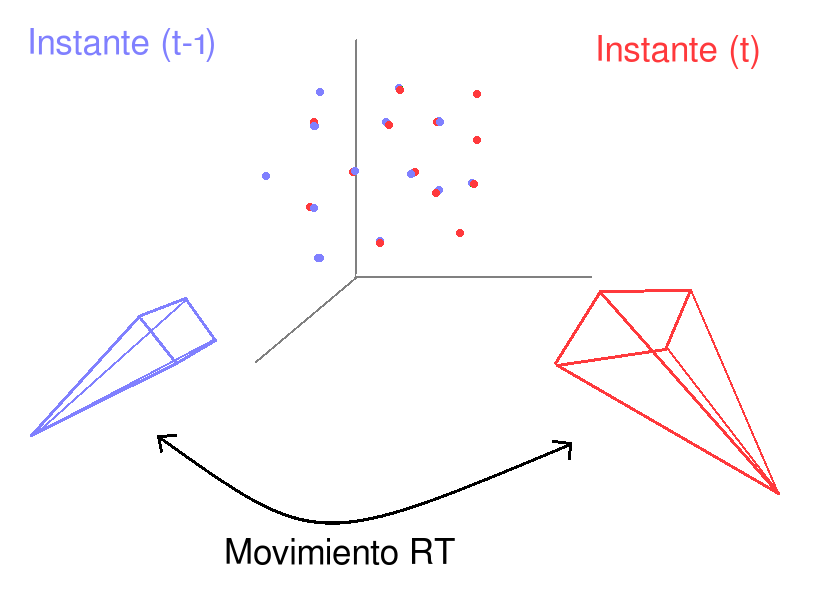
\includegraphics[scale=0.4]{Figures/movement-rt.png}
\decoRule
\caption[movement-rt]{Cálculo visual de movimiento en coordenadas absolutas.}
\label{fig:movementRt}
\end{figure}

Esos puntos comunes son por tanto los utilizados para el cálculo de movimiento. Provenientes del emparejamiento entre píxeles de las imágenes del bloque anterior.

Como entrada en este bloque tendremos:

\begin{enumerate}
\item \underline{Los puntos relativos} provenientes de la cámara en el instante $(t)$.
\item \underline{Los puntos absolutos} correspondientes al instante $(t-1)$.
\end{enumerate}

La nube de puntos guardada será almacenada en un vector del siguiente tipo:

\begin{lstlisting}[style=CStyle]
    struct myPoint {
      int x;
      int y;
      jderobot::RGBPoint rgbPoint;
    };
    std::vector<myPoint> myPrevPoints;
\end{lstlisting}

Donde se guardarán los píxeles y su correspondiente punto 3D en coordenadas absolutas, calculado de la iteración anterior. Con esto conseguimos la Matriz RT con un desplazamiento absoluto.

Para los cálculos de la matriz RT se ha usado la librería \textit{Eigen} con la descomposición en valores singulares (\textbf{SVD}), ya que permite resolver sistemas sobredimensionados. En concreto se ha usado la clase \textit{JacobiSVD} para la descomposición de una matriz rectangular.

Partiendo de la nube de puntos en coordenadas absolutas (mundo) del instante $(n-1)$ y la nube de puntos en coordenadas relativas (cam) en el instante $(n)$; se calcula la matriz RT de la camara con respecto al mundo:

\begin{equation}
RT_{cam}^{mundo}\cdot P_{pto(n-1)}^{mundo}=P_{pto(n)}^{cam}
\end{equation}

Del mismo modo, para calcular la nube de puntos del instante actual y con coordenadas absolutas solo se tendrá que multiplicar por la inversa de la matriz calculada:

\begin{equation}
\left(RT_{cam}^{mundo}\right)^{-1}\cdot P_{pto(n)}^{cam}=P_{pto(n)}^{mundo}
\end{equation}

Una vez llegados a este punto se guarda el resultado necesario para los cálculos de la siguiente iteración:

\begin{equation}
P_{pto(n)}^{mundo}\longrightarrow P_{pto(n-1)}^{mundo}
\end{equation}

\subsection{Optimización}

El cálculo de movimiento ha sido uno de los puntos en los que se ha encontrado más problema ya que el error es acumulativo y una iteración con un error demasiado grande produce que en los siguientes instantes el cálculo sea erróneo. Por ello, hay que asegurarse de que todos los datos que vienen de los anteriores bloques, vengan con el menor error posible.

Para corregir el error en esta fase se ha optado por añadir dos filtros:

\begin{itemize}
\item Deshacer el cálculo con demasiado error espacial y de reproyección.
\item Implementación de \textbf{RANSAC}.
\end{itemize}

Para el error espacial se ha medido la distancia entre los mismos puntos en el sistema de referencia absoluto para los intantes $(n-1)$ y $(n)$. 

Para el error de reproyección se mide la distancia entre píxeles de los diferentes instantes. Se calcula con \textit{Progeo} la posición del nuevo píxel en el instante anterior para poder calcular la distancia para una misma imágen.

Si la distancia total es muy grande se desecha el cálculo y se comienza con otra instante de tiempo

La implementación con RANSAC se compone de 3 fases:

\begin{enumerate}
\item De los puntos emparejados se selecciona un porcentaje aleatorio
\item El cálculo RT se repite tantas veces como se desee
\item De todas las iteraciones se busca la matriz que tenga menor error espacial o de reproyección.
\end{enumerate}

Se puede encontrar que hay dos variables a elección del usuario; el porcentaje aleatorio de selección de puntos (por defecto; 80\%) y el número de repeticiones de cálculo de la matriz (por defecto; 10).

Como se puede deducir, este algoritmo es muy robusto frente a valores espurios, ya que si se realiza el cálculo con alguno de estos valores se desechará el resultado.


%-----------------------------------
%	SECTION Interfaz gráfica
%-----------------------------------
\section{Interfaz gráfica}

El componente desarrollado dispone de una interfaz gráfica en donde se pueden ver gráficamente los pasos realizados, así como el resultado de toda la lógica del sistema. Ha sido desarrollada con \textit{glade} y la apariencia se puede observar en la Figura~\ref{fig:supergui}.

\begin{figure}[th]
\centering
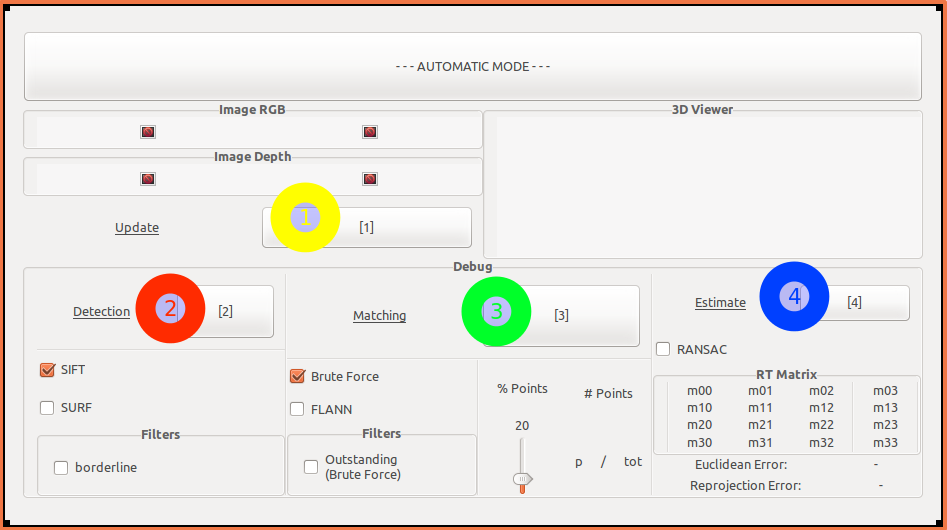
\includegraphics[scale=0.48]{Figures/super_gui.png}
\decoRule
\caption[supergui]{Captura del mapa de funcionalidades de la herramienta gráfica.}
\label{fig:supergui}
\end{figure}

La interfaz gráfica, basada en GTK, permite la realización  del procesado paso a paso o de manera automática: 

\begin{enumerate}
\item Actualización de imagen. (Figura~\ref{fig:gui1})

\begin{figure}[th]
\centering
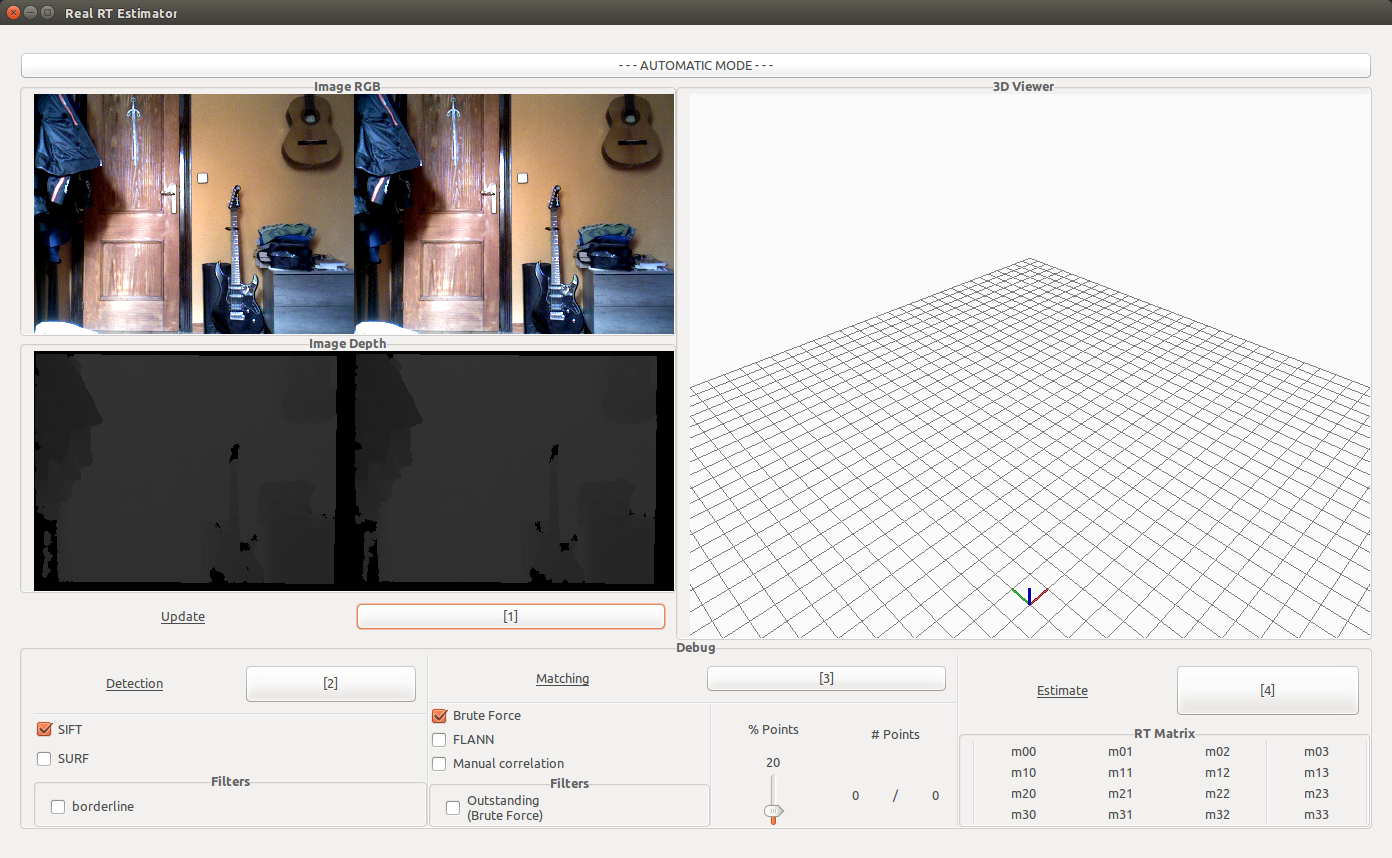
\includegraphics[scale=0.3]{Figures/gui1.png}
\decoRule
\caption[gui1]{Paso 1: Actualización de imagen.}
\label{fig:gui1}
\end{figure}

\item Detección de puntos. (Figura~\ref{fig:gui2})

\begin{figure}[th]
\centering
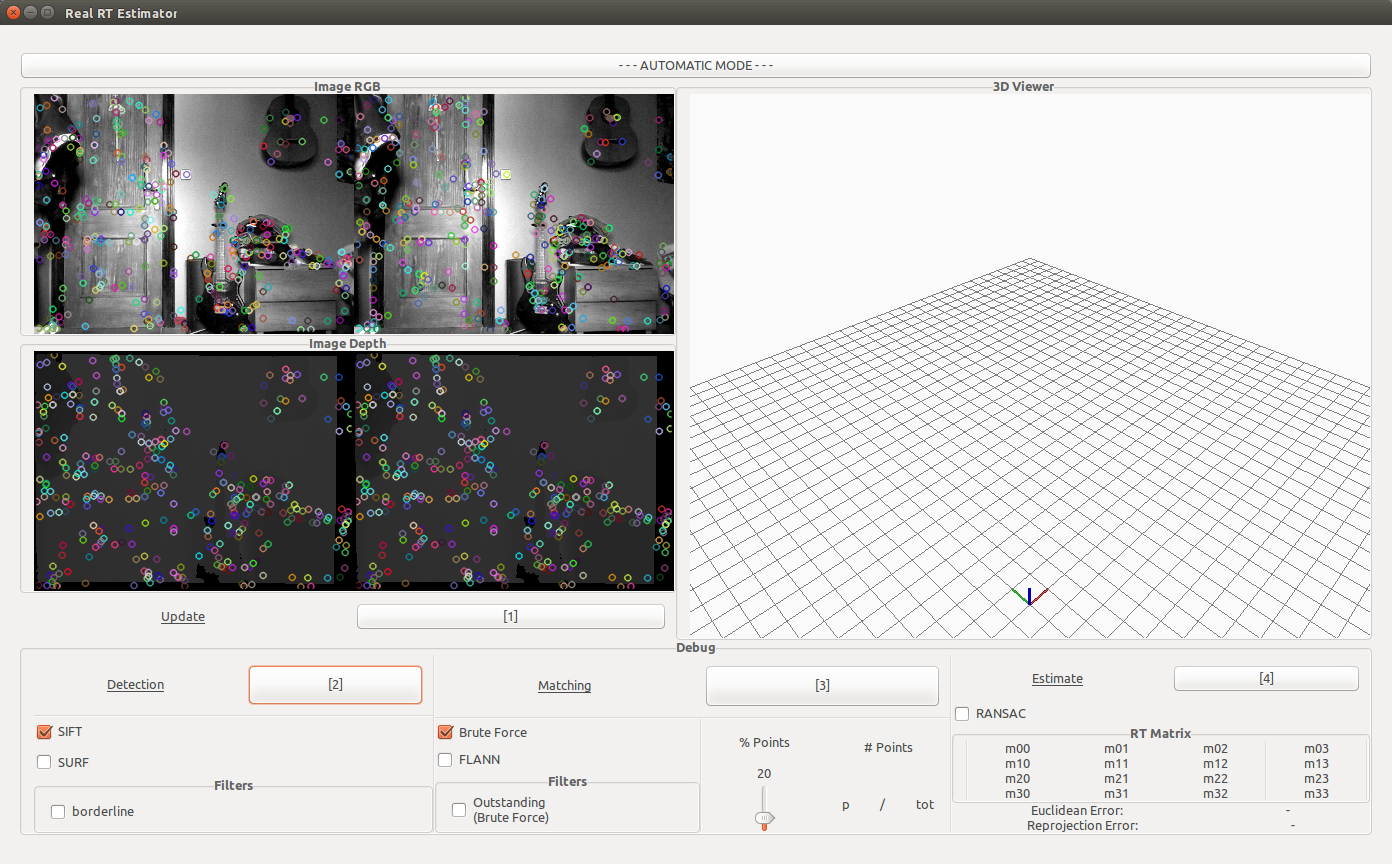
\includegraphics[scale=0.3]{Figures/gui2.png}
\decoRule
\caption[gui2]{Paso 2: Detección de puntos.}
\label{fig:gui2}
\end{figure}
 
\item Cálculo de emparejamientos. (Figura~\ref{fig:gui3})

\begin{figure}[th]
\centering
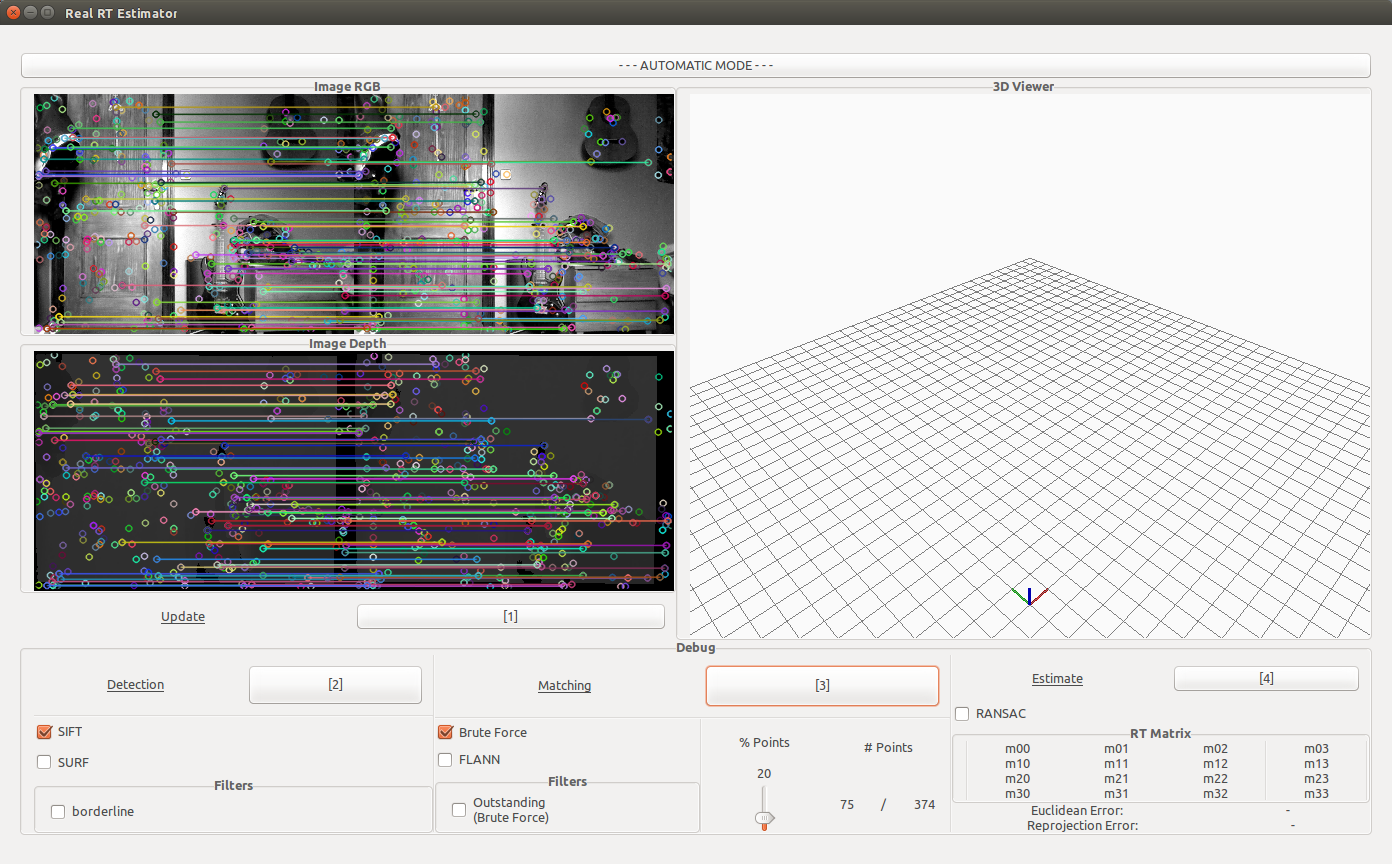
\includegraphics[scale=0.3]{Figures/gui3.png}
\decoRule
\caption[gui3]{Paso 3: Cálculo de emparejamientos.}
\label{fig:gui3}
\end{figure}

\item Estimación de la matriz. (Figura~\ref{fig:gui4})

\begin{figure}[th]
\centering
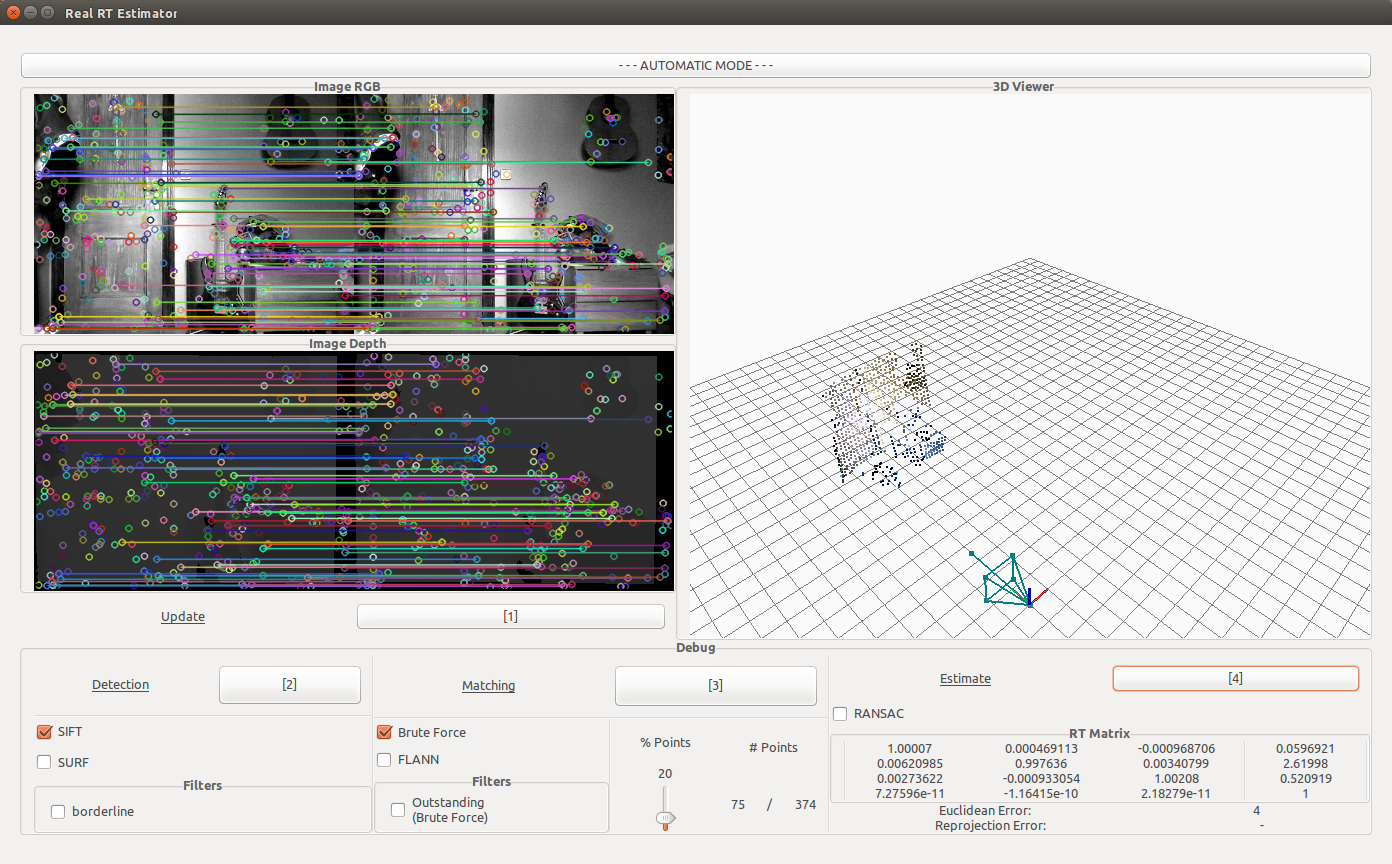
\includegraphics[scale=0.3]{Figures/gui4.png}
\decoRule
\caption[gui4]{Paso 4: Estimación de la matriz.}
\label{fig:gui4}
\end{figure}

\end{enumerate}

La herramienta permite, además, la modificación de algunos parámetros de configuración, como pueden ser la elección algortimos o filtros, así como el porcentaje de puntos emparejamientos a calcular.

Por último se ha implementado un visor 3D, donde se representa toda la información tridimensional para el sistema de referencia absoluto.
%% Chapter Template

\chapter{Experimentos}

\label{Chapter5} % Change X to a consecutive number; for referencing this chapter elsewhere, use \ref{ChapterX}

En este capítulo se detallarán las pruebas realizadas, con el objetivo de validar la solución propuesta en este trabajo. Además se comprobarán las diferentes configuraciones desarrolladas y se evaluarán sus prestaciones con los costes temporales. Estos experimentos han permitido depurar el componente para poder ajustar y mejorar la funcionalidad del mismo durante el desarrollo.

%-----------------------------------
%	SECTION Validación experimental
%-----------------------------------
\section{Validación experimental}

El entorno de pruebas utilizado ha sido siempre un entorno real, trabajando con los datos en vivo proporcionados por OpenniServer que extrae la información directamente del sensor.

Se propone en esta sección validar el componente en las diferentes fases que lo componen: detección de puntos de interés, cálculo de emparejamientos y estimación de movimiento.

\subsection{Detección de puntos de interés}



\subsection{Cálculo de emparejamientos}


\subsubsection{Posición estática}
\subsubsection{Traslación}
\subsubsection{Rotación}


\subsection{Resolución 3D}

La resolución 3D o estimación de movimiento compone el último paso que completa una iteración del sistema, por lo que en esta etapa podremos ver el resultado final del movimiento entre varios fotogramas consecutivos.

Las pruebas mostrados a continuación son realizadas con un funcionamiento normal del componente y en un tiempo determinado. El objetivo de estos experimentos es comprobar el comportamiento del sistema para los diferentes tipos de traslaciones ($x$, $y$, y $z$) y rotaciones (\textit{pitch}, \textit{yaw}, \textit{roll}).

Para estas pruebas y las siguientes se hará uso del componente con el comportamiento automático activado, repitiendo así de manera autónoma cada ciclo de estimación 3D. También se ha optado, para añadir robustez, el filtro de sobresaliencia y RANSAC.

\subsubsection{Validación de la traslación}

En la siguiente subsección se harán pruebas para comprobar como se comporta el sistema ante la traslación. Se moverá la cámara a lo largo de los tres ejes ($x$, $y$ y $z$) (Figura~\ref{fig:xyz}).

\begin{figure}[th]
\centering
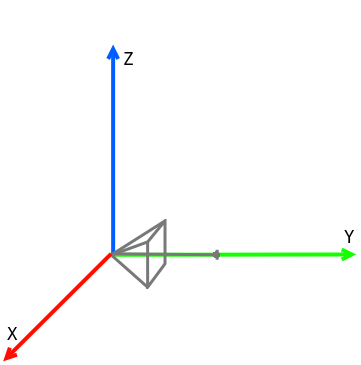
\includegraphics[scale=0.3]{Figures/xyz.png}
\decoRule
\caption[Ejes de coordenadas $x$, $y$ y $z$]{Ejes de coordenadas $x$, $y$ y $z$, con la orientación de la cámara.}
\label{fig:xyz}
\end{figure}

Para estas pruebas se va a utilizar el mismo entorno de trabajo por lo que el punto de partida será el que se muestra en la Figura~\ref{fig:init}.

\begin{figure}[th]
\centering
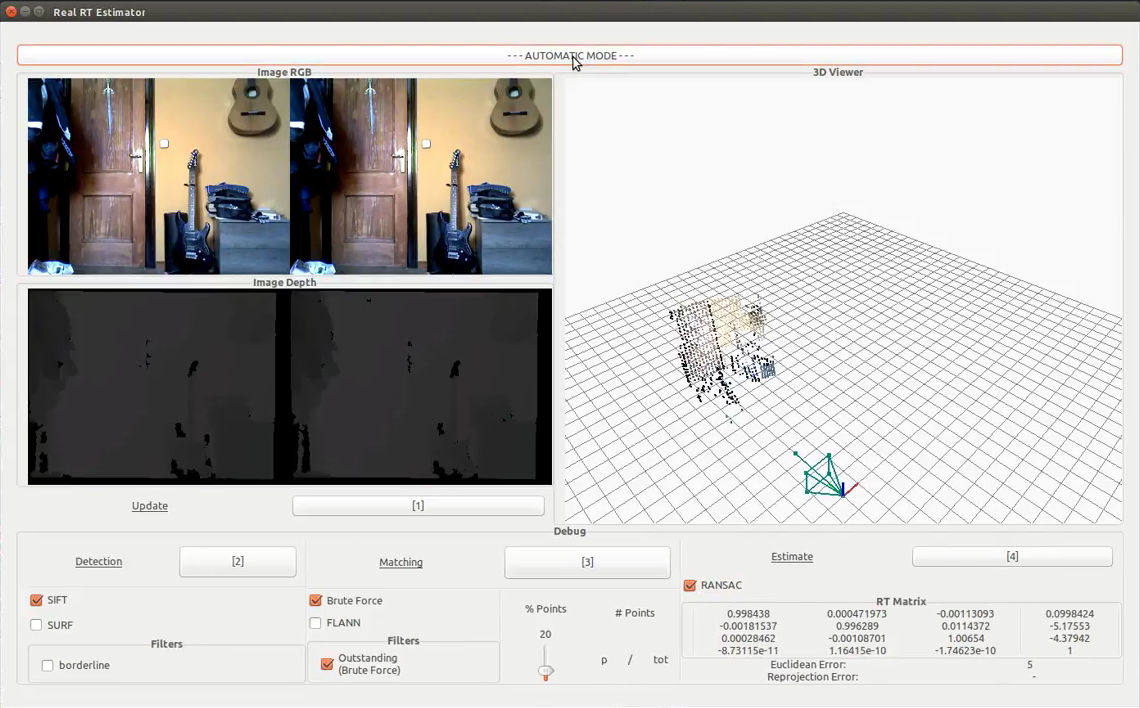
\includegraphics[scale=0.3]{Figures/tests/init.png}
\decoRule
\caption[Punto de partida para las pruebas de traslación y rotación]{Punto de partida para las pruebas realizadas.}
\label{fig:init}
\end{figure}

En la Figura~\ref{fig:axis-y} se muestra la estimación de movimiento sobre el eje $y$. El desplazamiento se ha intentado hacer lo más recto posible y el recorrido se muestra como estela en el visor 3D del componente. En ambas capturas se puede ver la ida y la vuelta recorriendo por cada una 1.5 metros aproximadamente. Después se ha vuelto a la posición de origen del movimiento.

\begin{figure}[th]
\centering
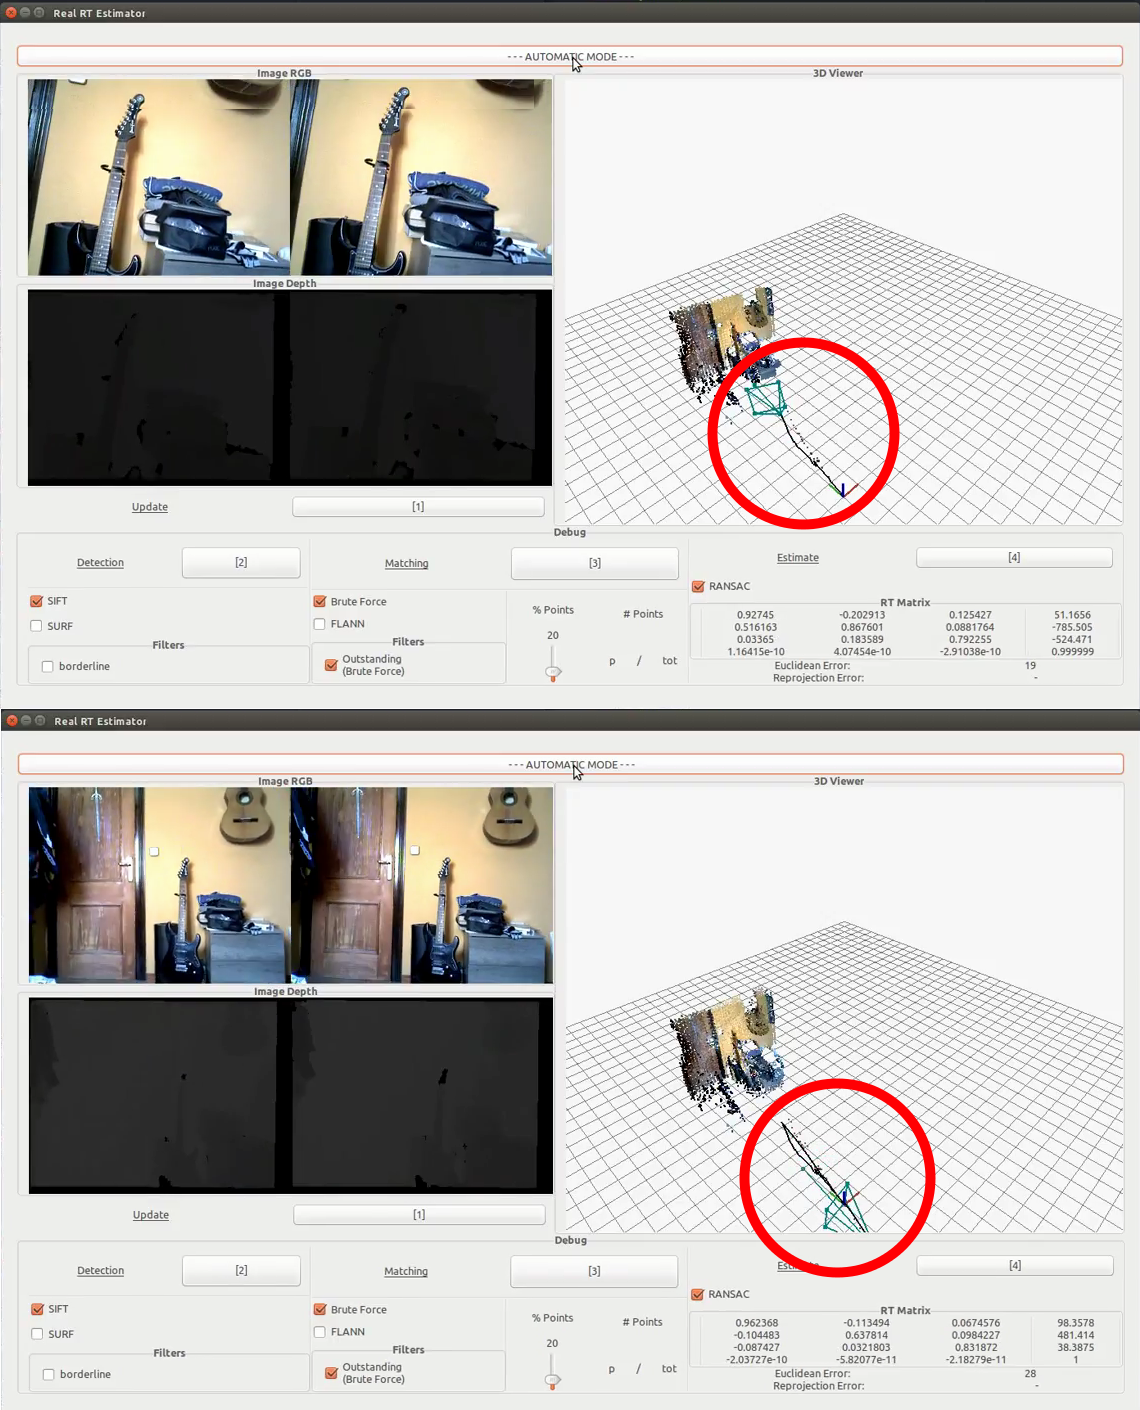
\includegraphics[scale=0.3]{Figures/tests/axis-y.png}
\decoRule
\caption[Prueba con desplazamiento en el eje $y$]{Prueba con desplazamiento en el eje $y$.}
\label{fig:axis-y}
\end{figure}

Se puede observar, después de aproximadamente 100 iteraciones, como ha afectado el error a la estimación al volver el sensor al origen.

En la Figura~\ref{fig:axis-xz} se puede ver el efecto de la traslación en los ejes $x$ y $z$ respectivamente. Se ve como el error en estos ejes es menor, percibiendo oscilaciones en su mayor parte únicamente en el eje $y$. La validación del eje $x$ se ha realizado sobre una mesa recorriendo 1 metro, por lo que no se obtiene desplazamiento en $z$. En cuanto a las pruebas del eje $z$ se aprecia un balanceo en $x$ debido al movimiento vertical de la mano ya que no ha seguido una trayectoria recta.

\begin{figure}[th]
\centering
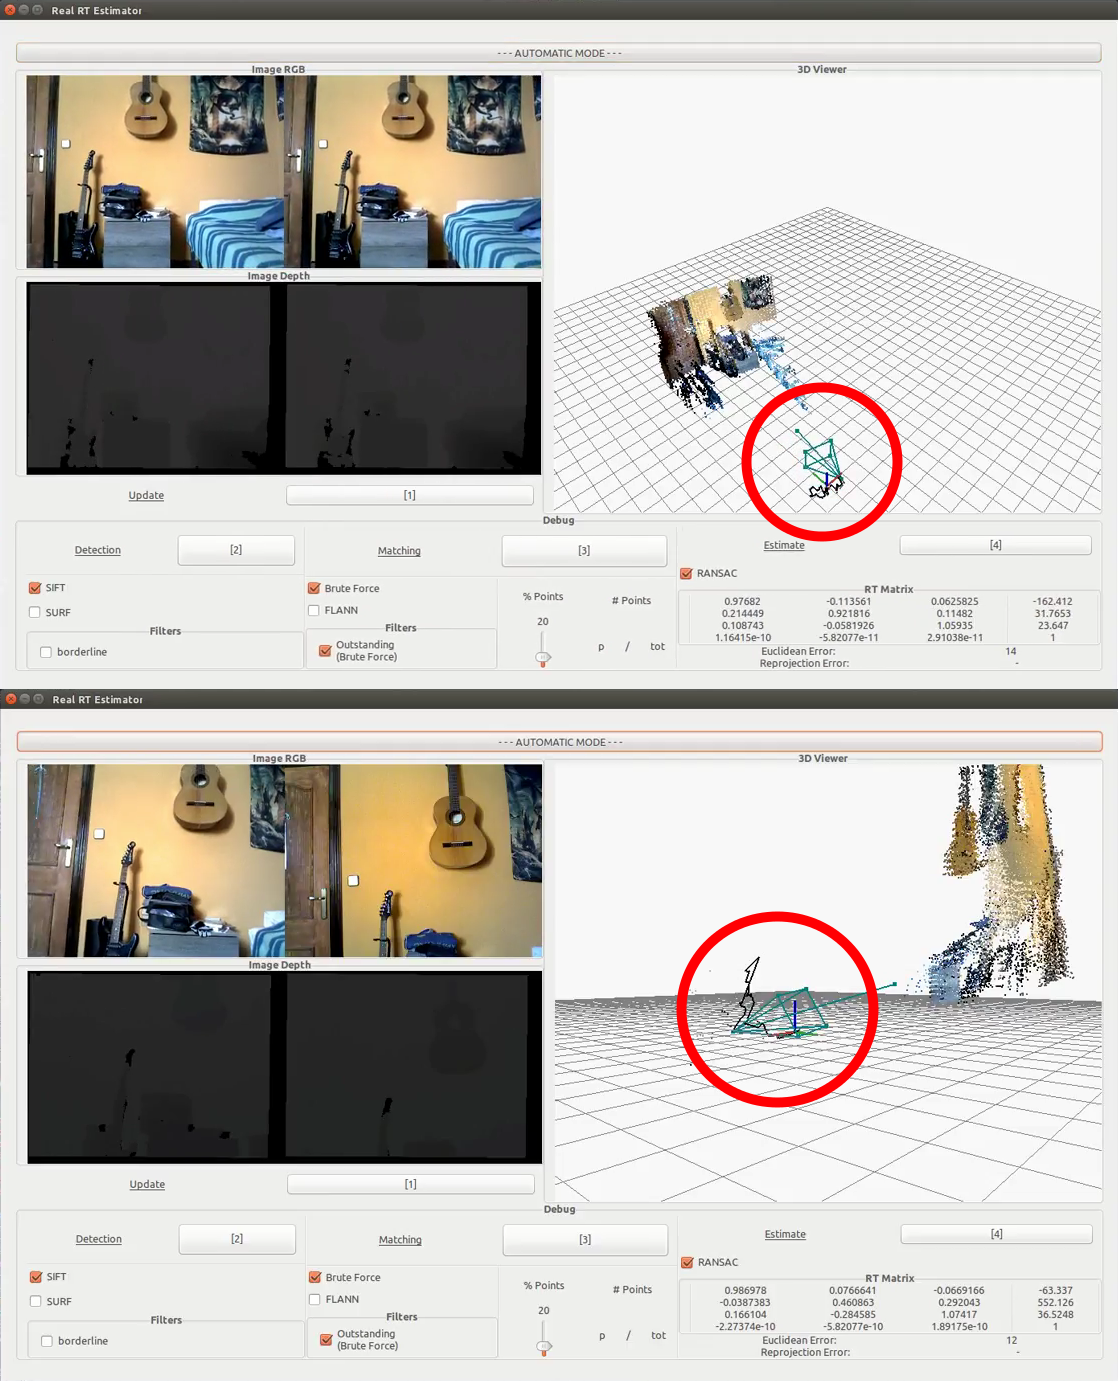
\includegraphics[scale=0.3]{Figures/tests/axis-x-z.png}
\decoRule
\caption[Prueba con desplazamiento en los ejes $x$ y $z$]{Prueba con desplazamiento en los ejes $x$ y $z$.}
\label{fig:axis-xz}
\end{figure}

Los resultados son aceptables en la estimación, no se consigue un cierre de trayectoria perfecto pero se acerca. Pensando que se ha aplicado una traslación de más de 1 metro el error final obtenido se puede medir en centímetros, acentuándose más para el eje $y$ correspondiente al perpendicular al plano imagen y el que se obtiene de la imagen de profundidad.

Como vimos en el capítulo \ref{Chapter3} la información de profundidad del sensor no es perfecta y tiene un pequeño margen de error. A parte de tener un rango de distancias óptimo establecido por el fabricante (\textit{0.8 to 3.5 m}), fuera de este rango la imagen de profundidad empieza a empeorar drásticamente y por consiguiente la estimación de movimiento.

\subsubsection{Validación de la Rotación}
\subsubsection{Validación de trayectorias complejas}

\subsection{Error estático}

El error estático muestra el ruido blanco que se esconde detrás de la resolución 3D en tiempo real. Como se va a poder observar en esta sección, el ruido estático es inevitable y no depende del algoritmo a utilizar. Sin embargo, en el siguiente capítulo, en el cual se propone posibles mejoras y líneas futuras, se verán métodos para poder elimnarlo en mayor o menor medida.

En las siguientes Figuras (\ref{fig:static1}, \ref{fig:static2}, \ref{fig:static3}) se puede ver un ejemplo de este error para diferentes configuraciones. Como se puede interpretar es un error que está presente en todos los casos.

\begin{figure}[th]
\centering
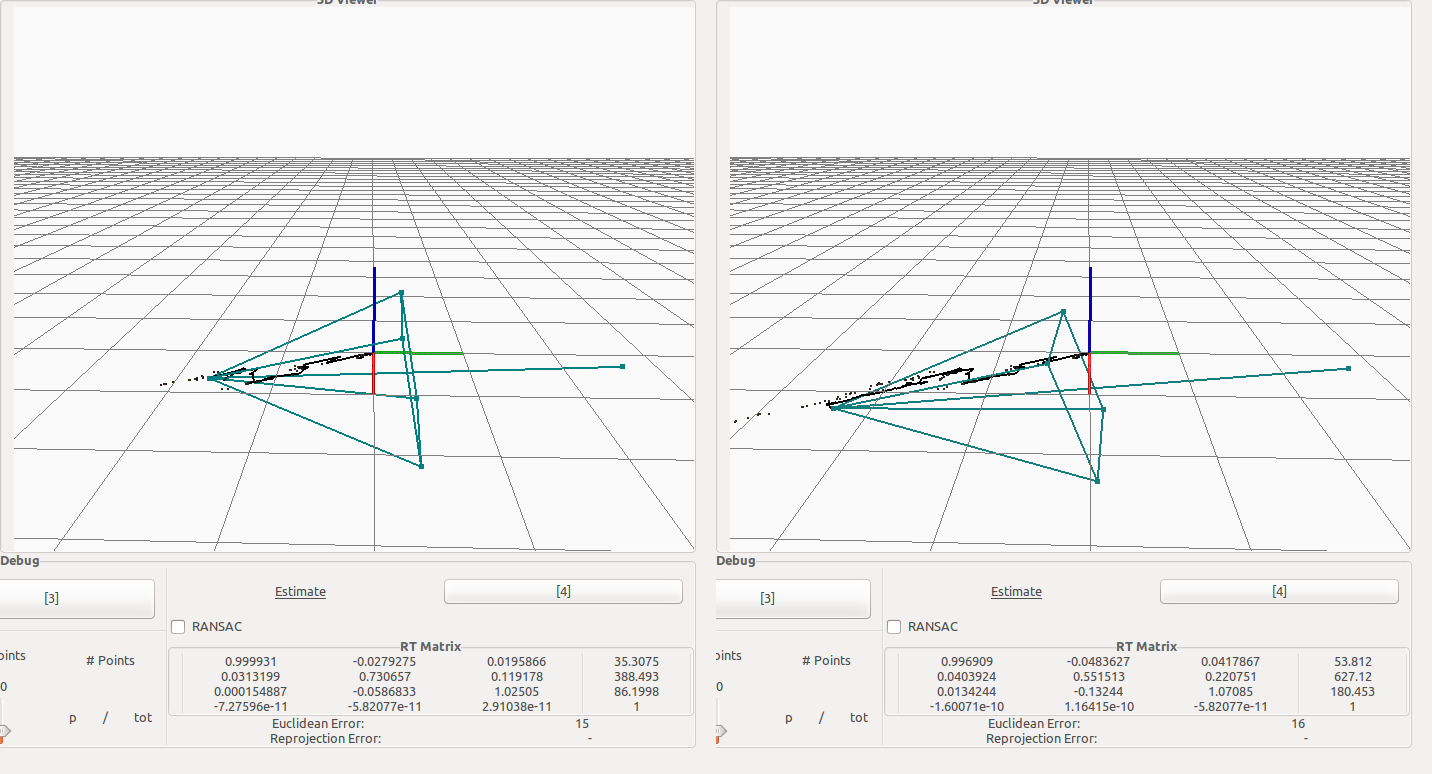
\includegraphics[scale=0.3]{Figures/tests/static-surf-flann_2.png}
\decoRule
\caption[Ruido estático, con SURF y FLANN]{Ruido estático después de 30 y 60 segundos, con SURF y FLANN.}
\label{fig:static1}
\end{figure}

\begin{figure}[th]
\centering
\includegraphics[scale=0.3]{Figures/tests/static-filter_2.png}
\decoRule
\caption[Ruido estático, con SIFT, Fuerza Bruta y filtros]{Ruido estático después de 30 y 60 segundos, con SIFT, Fuerza Bruta y filtros.}
\label{fig:static2}
\end{figure}

\begin{figure}[th]
\centering
\includegraphics[scale=0.3]{Figures/tests/static-ransac_2.png}
\decoRule
\caption[Ruido estático, con SIFT, Fuerza Bruta y RANSAC]{Ruido estático después de 30 y 60 segundos, con SIFT, Fuerza Bruta y RANSAC.}
\label{fig:static3}
\end{figure}

Las pruebas realizadas han sido capturadas a los 30 y 60 segundos respectivamente y la configuración aplicada se encuentra en la descripción de cada Figura.

Si analizamos las matrices RT obtenidas se puede observar que el eje en que más avanza el ruido es el eje $y$, al igual que pasaba en las pruebas de la sección anterior.


%-----------------------------------
%	SECTION Tiempos de procesado
%-----------------------------------
\section{Tiempos de procesado} 

%----------------------------------------------------------------------------------------
%	THESIS CONTENT - APPENDICES
%----------------------------------------------------------------------------------------


%----------------------------------------------------------------------------------------
%	BIBLIOGRAPHY
%----------------------------------------------------------------------------------------

\printbibliography[heading=bibintoc]

%----------------------------------------------------------------------------------------

\end{document}  
